% Options for packages loaded elsewhere
\PassOptionsToPackage{unicode}{hyperref}
\PassOptionsToPackage{hyphens}{url}
\PassOptionsToPackage{dvipsnames,svgnames*,x11names*}{xcolor}
%
\documentclass[
]{article}
\usepackage{lmodern}
\usepackage{setspace}
\usepackage{amssymb,amsmath}
\usepackage{ifxetex,ifluatex}
\ifnum 0\ifxetex 1\fi\ifluatex 1\fi=0 % if pdftex
  \usepackage[T1]{fontenc}
  \usepackage[utf8]{inputenc}
  \usepackage{textcomp} % provide euro and other symbols
\else % if luatex or xetex
  \usepackage{unicode-math}
  \defaultfontfeatures{Scale=MatchLowercase}
  \defaultfontfeatures[\rmfamily]{Ligatures=TeX,Scale=1}
\fi
% Use upquote if available, for straight quotes in verbatim environments
\IfFileExists{upquote.sty}{\usepackage{upquote}}{}
\IfFileExists{microtype.sty}{% use microtype if available
  \usepackage[]{microtype}
  \UseMicrotypeSet[protrusion]{basicmath} % disable protrusion for tt fonts
}{}
\makeatletter
\@ifundefined{KOMAClassName}{% if non-KOMA class
  \IfFileExists{parskip.sty}{%
    \usepackage{parskip}
  }{% else
    \setlength{\parindent}{0pt}
    \setlength{\parskip}{6pt plus 2pt minus 1pt}}
}{% if KOMA class
  \KOMAoptions{parskip=half}}
\makeatother
\usepackage{xcolor}
\IfFileExists{xurl.sty}{\usepackage{xurl}}{} % add URL line breaks if available
\IfFileExists{bookmark.sty}{\usepackage{bookmark}}{\usepackage{hyperref}}
\hypersetup{
  pdftitle={Integrated multi-omics analysis reveals Lactobacillus anti-inflammatory process in vaginal tissue},
  pdfkeywords={pandoc, r markdown, knitr},
  colorlinks=true,
  linkcolor=blue,
  filecolor=Maroon,
  citecolor=Blue,
  urlcolor=Blue,
  pdfcreator={LaTeX via pandoc}}
\urlstyle{same} % disable monospaced font for URLs
\usepackage[margin=1in]{geometry}
\usepackage{longtable,booktabs}
% Correct order of tables after \paragraph or \subparagraph
\usepackage{etoolbox}
\makeatletter
\patchcmd\longtable{\par}{\if@noskipsec\mbox{}\fi\par}{}{}
\makeatother
% Allow footnotes in longtable head/foot
\IfFileExists{footnotehyper.sty}{\usepackage{footnotehyper}}{\usepackage{footnote}}
\makesavenoteenv{longtable}
\usepackage{graphicx}
\makeatletter
\def\maxwidth{\ifdim\Gin@nat@width>\linewidth\linewidth\else\Gin@nat@width\fi}
\def\maxheight{\ifdim\Gin@nat@height>\textheight\textheight\else\Gin@nat@height\fi}
\makeatother
% Scale images if necessary, so that they will not overflow the page
% margins by default, and it is still possible to overwrite the defaults
% using explicit options in \includegraphics[width, height, ...]{}
\setkeys{Gin}{width=\maxwidth,height=\maxheight,keepaspectratio}
% Set default figure placement to htbp
\makeatletter
\def\fps@figure{htbp}
\makeatother
\setlength{\emergencystretch}{3em} % prevent overfull lines
\providecommand{\tightlist}{%
  \setlength{\itemsep}{0pt}\setlength{\parskip}{0pt}}
\setcounter{secnumdepth}{5}
\usepackage{fancyhdr}
\pagestyle{fancy}
\fancyhead[L]{XXXXXXXXXXX et al.}
\fancyhead[R]{MANUSCRIPT SHORT TITLE}
\usepackage{lineno}
\linenumbers
\usepackage{booktabs}
\usepackage{longtable}
\usepackage{array}
\usepackage{multirow}
\usepackage{wrapfig}
\usepackage{float}
\usepackage{colortbl}
\usepackage{pdflscape}
\usepackage{tabu}
\usepackage{threeparttable}
\usepackage{threeparttablex}
\usepackage[normalem]{ulem}
\usepackage{makecell}
\usepackage{xcolor}
\ifluatex
  \usepackage{selnolig}  % disable illegal ligatures
\fi
\newlength{\cslhangindent}
\setlength{\cslhangindent}{1.5em}
\newenvironment{cslreferences}%
  {}%
  {\par}

\title{Integrated multi-omics analysis reveals Lactobacillus anti-inflammatory process in vaginal tissue}
\usepackage{etoolbox}
\makeatletter
\providecommand{\subtitle}[1]{% add subtitle to \maketitle
  \apptocmd{\@title}{\par {\large #1 \par}}{}{}
}
\makeatother
\subtitle{A demonstration of Rmarkdown using Herman Bumpus' data}
\author{Author One\textsuperscript{1},
Author Two\textsuperscript{2},
Author Three\textsuperscript{1,2}}
\date{March 12, 2021}

\begin{document}
\maketitle

\setstretch{1.5}
\footnotetext[1]{University of Nowhere}
\footnotetext[2]{University of Somewhere}
\footnotetext[3]{University of Lalaland}

\hypertarget{abstract}{%
\section{Abstract}\label{abstract}}

Abstract Abstract Abstract Abstract Abstract Abstract Abstract Abstract Abstract Abstract Abstract Abstract Abstract Abstract Abstract Abstract Abstract Abstract Abstract Abstract Abstract Abstract Abstract Abstract Abstract Abstract Abstract Abstract Abstract Abstract Abstract Abstract Abstract Abstract Abstract Abstract Abstract Abstract Abstract Abstract Abstract Abstract Abstract Abstract Abstract Abstract Abstract Abstract Abstract Abstract Abstract Abstract Abstract Abstract Abstract Abstract Abstract Abstract Abstract Abstract Abstract Abstract Abstract Abstract Abstract Abstract Abstract Abstract Abstract Abstract Abstract Abstract Abstract Abstract Abstract Abstract Abstract Abstract Abstract Abstract Abstract Abstract Abstract Abstract Abstract Abstract Abstract Abstract Abstract Abstract Abstract Abstract Abstract Abstract Abstract Abstract Abstract Abstract Abstract Abstract Abstract Abstract Abstract Abstract Abstract Abstract Abstract Abstract Abstract Abstract Abstract Abstract Abstract Abstract Abstract Abstract Abstract Abstract Abstract Abstract Abstract Abstract Abstract Abstract Abstract Abstract Abstract Abstract Abstract Abstract Abstract Abstract Abstract Abstract Abstract Abstract Abstract Abstract Abstract Abstract Abstract Abstract Abstract Abstract Abstract Abstract Abstract Abstract Abstract Abstract Abstract Abstract Abstract Abstract Abstract Abstract Abstract Abstract Abstract Abstract Abstract Abstract Abstract Abstract Abstract Abstract Abstract Abstract Abstract Abstract Abstract Abstract Abstract Abstract Abstract Abstract
test test test

\clearpage

\hypertarget{introduction}{%
\section{Introduction}\label{introduction}}

Introduction Introduction Introduction Introduction Introduction Introduction Introduction Introduction Introduction Introduction Introduction Introduction Introduction Introduction Introduction Introduction Introduction Introduction Introduction Introduction Introduction Introduction Introduction Introduction Introduction Introduction Introduction Introduction Introduction Introduction Introduction Introduction Introduction Introduction Introduction Introduction (\textsuperscript{\protect\hyperlink{ref-Johnston1972}{1}}), Introduction Introduction Introduction Introduction Introduction Introduction Introduction Introduction Introduction Introduction Introduction Introduction Introduction Introduction Introduction Introduction Introduction Introduction Introduction Introduction Introduction Introduction Introduction Introduction Introduction \textbf{Introduction Introduction} \emph{Introduction} Introduction (\textsuperscript{\protect\hyperlink{ref-Darwin1859}{2}}\textsuperscript{,}\textsuperscript{\protect\hyperlink{ref-Bumpus1898}{3}}) .

Problem / question to answer

\clearpage

\hypertarget{results}{%
\section{Results}\label{results}}

\textbf{Joint analysis of vaginal microbiome reveals distinct patient subgroups}

To understand the longitudinal and tissue-specific microbiome profile in vaginal samples, 111 adult female sex workers were enrolled in {[}\ldots{]}. Among those, 14 were previously tested positive for HIV during the cohort's sampling procedure. {[}Describe here what was done and when, which samples, which tissues{]}.

To be able to better undertand the differences in microbiome profile across all datasets collected, we performed a joint graph-based clustering analysis in order to identify co-regulated bacterial communities (see ``Methods'' section for details). A total of 15 bacterial communities were identified.

Noticebly, bacterial community NA consisted only of Lactobacillus species (**).

Patients were thus subdivided into 8 groups,

Results Results Results Results Results Results Results Results Results Results Results Results Results Results Results Results Results Results Results Results Results Results Results Results Results Results Results Results Results Results Results Results Results Results Results Results Results Results Results Results Results Results Results Results Results Results Results Results Results Results Results Results Results Results Results Results Results Results Results Results Results Results Results Results Results Results Results Results Results Results Results Results Results Results Results Results Results Results Results Results Results Results Results Results Results Results Results Results Results Results Results Results Results Results Results Results Results Results Results Results Results Results Results Results Results Results Results Results Results Results Results Results Results Results Results Results Results Results Results Results Results Results Results Results Results Results Results Results Results Results Results Results Results Results Results Results Results Results Results Results Results Results Results Results Results Results Results Results Results Results Results Results Results Results Results Results Results Results Results Results Results Results Results Results Results Results Results Results Results Results Results Results Results Results Results Results Results Results Results Results Results Results Results Results Results Results Results Results Results Results Results Results Results Results Results Results Results Results Results Results Results Results Results Results Results Results Results Results Results Results Results Results Results Results Results Results Results Results Results Results Results Results Results Results Results Results Results Results Results Results Results Results Results Results Results Results Results Results Results Results Results Results Results Results Results Results Results Results Results Results Results Results Results Results Results Results Results Results Results Results Results Results Results Results Results Results Results Results Results Results Results Results Results Results Results Results Results Results Results Results Results Results Results Results Results Results Results Results Results Results Results Results Results Results Results Results Results Results Results Results Results Results Results Results Results Results Results Results Results Results Results Results Results Results Results Results Results Results Results Results Results Results Results Results Results Results Results Results Results Results Results Results Results Results Results Results Results Results Results Results Results Results Results Results Results Results Results Results Results Results Results Results Results Results Results Results Results Results Results Results Results Results Results Results Results Results Results Results Results Results Results Results Results Results Results Results Results Results Results Results Results Results Results Results Results Results Results Results Results Results Results Results Results Results Results Results Results Results Results Results Results Results Results Results Results

\clearpage

\textbf{Indentification of bacterial communities metabolic processes linked to Lactobacilli}

Results Results Results Results Results Results Results Results Results Results Results Results Results Results Results Results Results Results Results Results Results Results Results Results Results Results Results Results Results Results Results Results Results Results Results Results Results Results Results Results Results Results Results Results Results Results Results Results Results Results Results Results Results Results Results Results Results Results Results Results Results Results Results Results Results Results Results Results Results Results Results Results Results Results Results Results Results Results Results Results Results Results Results Results Results Results Results Results Results Results Results Results Results Results Results Results Results Results Results Results Results Results Results Results Results Results Results Results Results Results Results Results Results Results Results Results Results Results Results Results Results Results Results Results Results Results Results Results Results Results Results Results Results Results Results Results Results Results Results Results Results Results Results Results Results Results Results Results Results Results Results Results Results Results Results Results Results Results Results Results Results Results Results Results Results Results Results Results Results Results Results Results Results Results Results Results Results Results Results Results Results Results Results Results Results Results Results Results Results Results Results Results Results Results Results Results Results Results Results Results Results Results Results Results Results Results Results Results Results Results Results Results Results Results Results Results Results Results Results Results Results Results Results Results Results Results Results Results Results Results Results Results Results Results Results Results Results Results Results Results Results Results Results Results Results Results Results Results Results Results Results Results Results Results Results Results Results Results Results Results Results Results Results Results Results Results Results Results Results Results Results Results Results Results Results Results Results Results Results Results Results Results Results Results Results Results Results Results Results Results Results Results Results Results Results Results Results Results Results Results Results Results Results Results Results Results Results Results Results Results Results Results Results Results Results Results Results Results Results Results Results Results Results Results

\clearpage

\textbf{Indentification of bacterial communities metabolic processes linked to Lactobacilli}

Results Results Results Results Results Results Results Results Results Results Results Results Results Results Results Results Results Results Results Results Results Results Results Results Results Results Results Results Results Results Results Results Results Results Results Results Results Results Results Results Results Results Results Results Results Results Results Results Results Results Results Results Results Results Results Results Results Results Results Results Results Results Results Results Results Results Results Results Results Results Results Results Results Results Results Results Results Results Results Results Results Results Results Results Results Results Results Results Results Results Results Results Results Results Results Results Results Results Results Results Results Results Results Results Results Results Results Results Results Results Results Results Results Results Results Results Results Results Results Results Results Results Results Results Results Results Results Results Results Results Results Results Results Results Results Results Results Results Results Results Results Results Results Results Results Results Results Results Results Results Results Results Results Results Results Results Results Results Results Results Results Results Results Results Results Results Results Results Results Results Results Results Results Results Results Results Results Results Results Results Results Results Results Results Results Results Results Results Results Results Results Results Results Results Results Results Results Results Results Results Results Results Results Results Results Results Results Results Results Results Results Results Results Results Results Results Results Results Results Results Results Results Results Results Results Results Results Results Results Results Results Results Results Results Results Results Results Results Results Results Results Results Results Results Results Results Results Results Results Results Results Results Results Results Results Results Results Results Results Results Results Results Results Results Results Results Results Results Results Results Results Results Results Results Results Results Results Results Results Results Results Results Results Results Results Results Results Results Results Results Results Results Results Results Results Results Results Results Results Results Results Results Results Results Results Results Results Results Results Results Results Results Results Results Results Results Results Results Results Results Results Results Results Results

\clearpage

\hypertarget{discussion}{%
\section{Discussion}\label{discussion}}

I have analysed data collected by Herman Bumpus\textsuperscript{\protect\hyperlink{ref-Bumpus1898}{3}} on the relationship between sparrow (\emph{Passer domesticus}) total length and surival following an unusually severe storm. I found that sparrows that died in the storm were longer than sparrows that survived, which suggests that higher sparrow body length decreased survival. Of course, it is not possible to definitively conclude a causal relationship between any aspect of body size and sparrow survival, and even the available data collected by Bumpus would permit a more thoughtful analysis than that conducted in this study (see \protect\hyperlink{appendix}{Appendix Table 1}).

Overall, this document demonstrates how high quality, professional looking documents can be written using Rmarkdown. The \href{https://github.com/StirlingCodingClub/Manuscripts_in_Rmarkdown/blob/master/ms.Rmd}{underlying code} for this manuscript is publicly available, along with \href{https://stirlingcodingclub.github.io/Manuscripts_in_Rmarkdown/Rmarkdown_notes.html}{accompanying notes} to understand how it was written. By using Rmarkdown to write manuscripts, authors can more easily use version control (e.g., git) throughout the writing process. The ability to easily integrate citations though BibTeX, LaTeX tools, and dynamic R code can also make writing much more efficient and more enjoyable. Further, obtaining the benefits of using Rmarkdown does not need to come with the cost of isolating colleagues who prefer to work with Word or LaTeX because Rmarkdown can easily be converted to these formats (in the case of Word, with the push of a button). By learning all of the tools used in this manuscript, readers should have all of the necessary knowledge to get started writing and collaborating in Rmarkdown.

\clearpage

\hypertarget{methods}{%
\section{Methods}\label{methods}}

\clearpage

\hypertarget{references}{%
\section{References}\label{references}}

\hypertarget{refs}{}
\begin{cslreferences}
\leavevmode\hypertarget{ref-Johnston1972}{}%
1. Johnston, R. F., Niles, D. M. \& Rohwer, S. A. Hermon bumpus and natural selection in the house sparrow \emph{Passer domesticus}. \emph{Evolution} \textbf{26}, 20--31 (1972).

\leavevmode\hypertarget{ref-Darwin1859}{}%
2. Darwin, C. \emph{The origin of species}. 495 (Penguin, 1859).

\leavevmode\hypertarget{ref-Bumpus1898}{}%
3. Bumpus, H. C. Eleventh lecture. The elimination of the unfit as illustrated by the introduced sparrow, \emph{Passer domesticus}. (A fourth contribution to the study of variation.). \emph{Biological Lectures: Woods Hole Marine Biological Laboratory} 209--225 (1898).
\end{cslreferences}

\clearpage

\hypertarget{appendix-table-1}{%
\section{Appendix Table 1}\label{appendix-table-1}}

An example table is shown below, which includes all of the variables collected by \protect\hyperlink{ref-Bumpus1898}{3} for the first 10 measured sparrows. The full data set can be found online in \href{https://github.com/StirlingCodingClub/Manuscripts_in_Rmarkdown/blob/master/data/Bumpus_data.csv}{GitHub}.

\clearpage

\hypertarget{figures-main}{%
\section{FIGURES (MAIN)}\label{figures-main}}

\hypertarget{figure-1}{%
\subsection{Figure 1}\label{figure-1}}

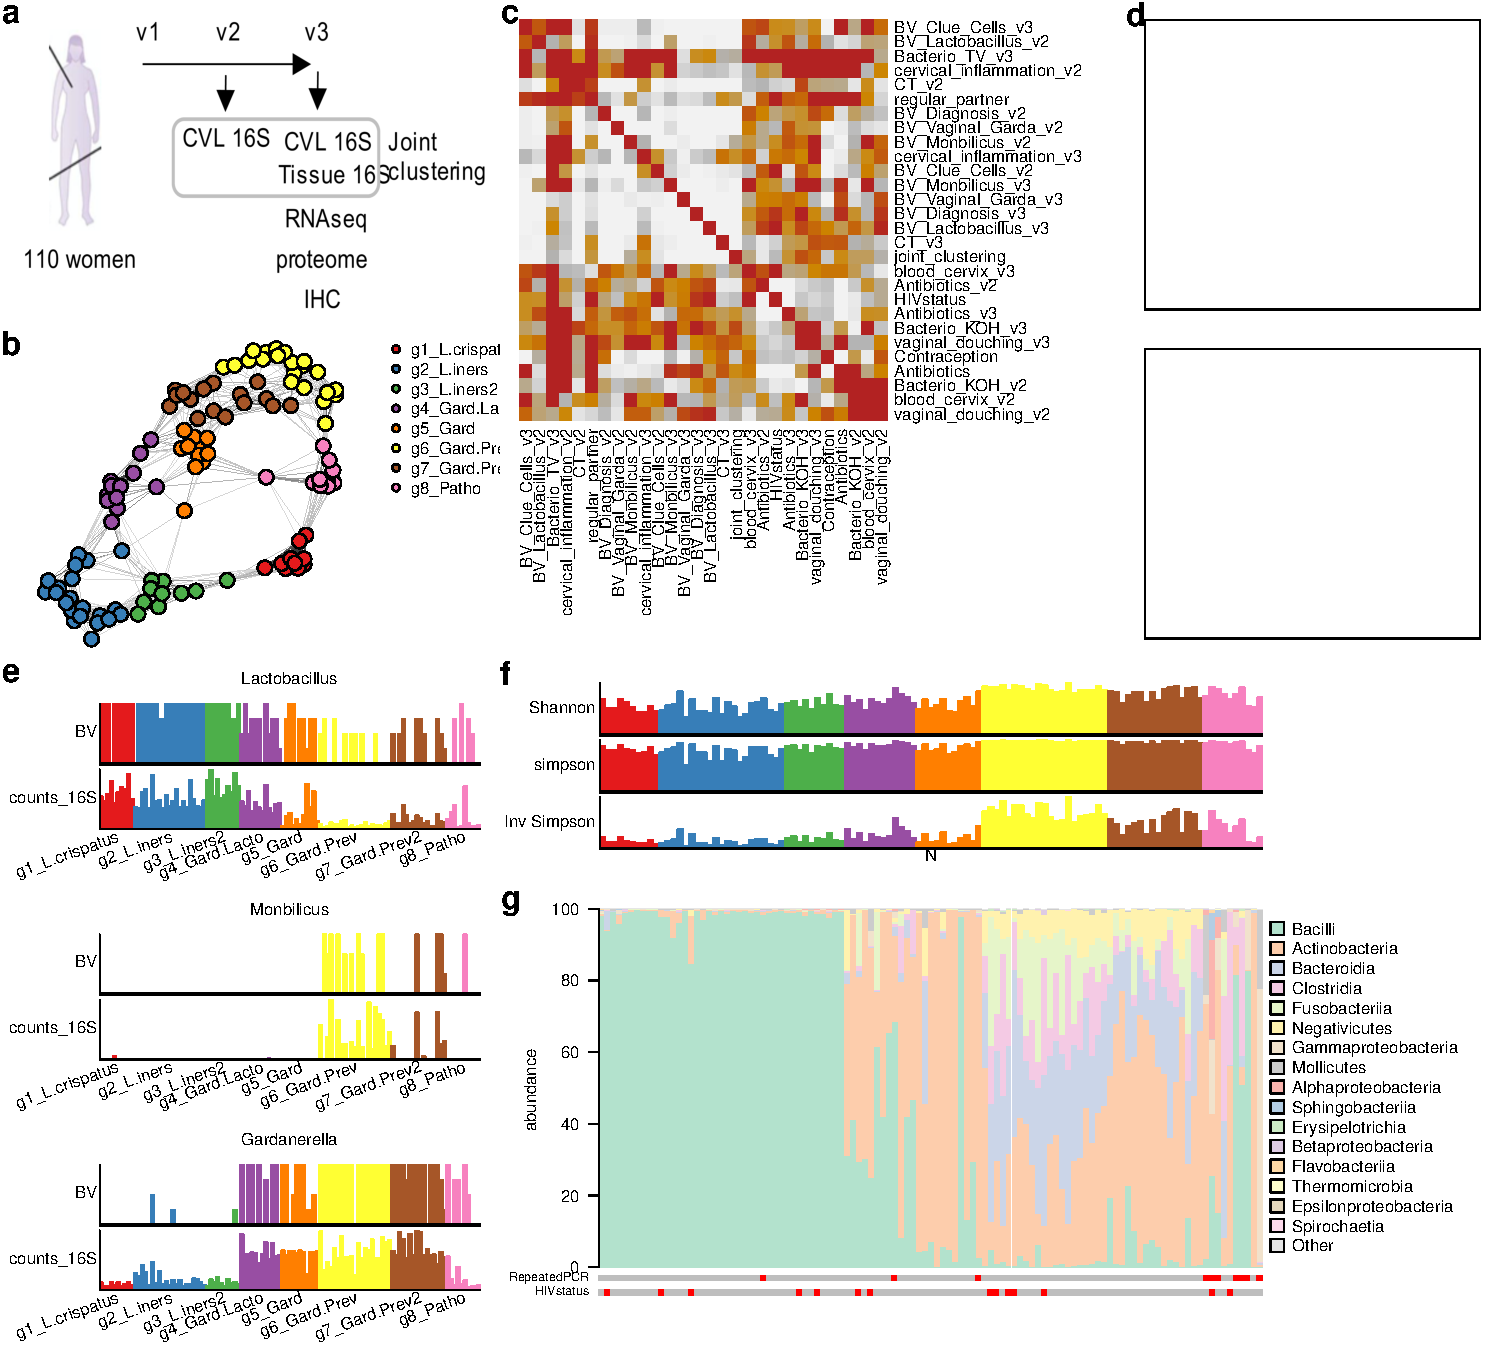
\includegraphics[width=1\linewidth]{manuscript_template_files/figure-latex/unnamed-chunk-5-1}

\textbf{Figure 1. Identification of patient groups.}
(\textbf{a}) Schematic representation of \#\#\#\#\#\#\#\#\#\# .
(\textbf{b}) Schematic representation of \#\#\#\#\#\#\#\#\#\# .
(\textbf{c}) Schematic representation of \#\#\#\#\#\#\#\#\#\# .
(\textbf{d}) Schematic representation of \#\#\#\#\#\#\#\#\#\# .

\clearpage

\hypertarget{figure-2}{%
\subsection{Figure 2}\label{figure-2}}

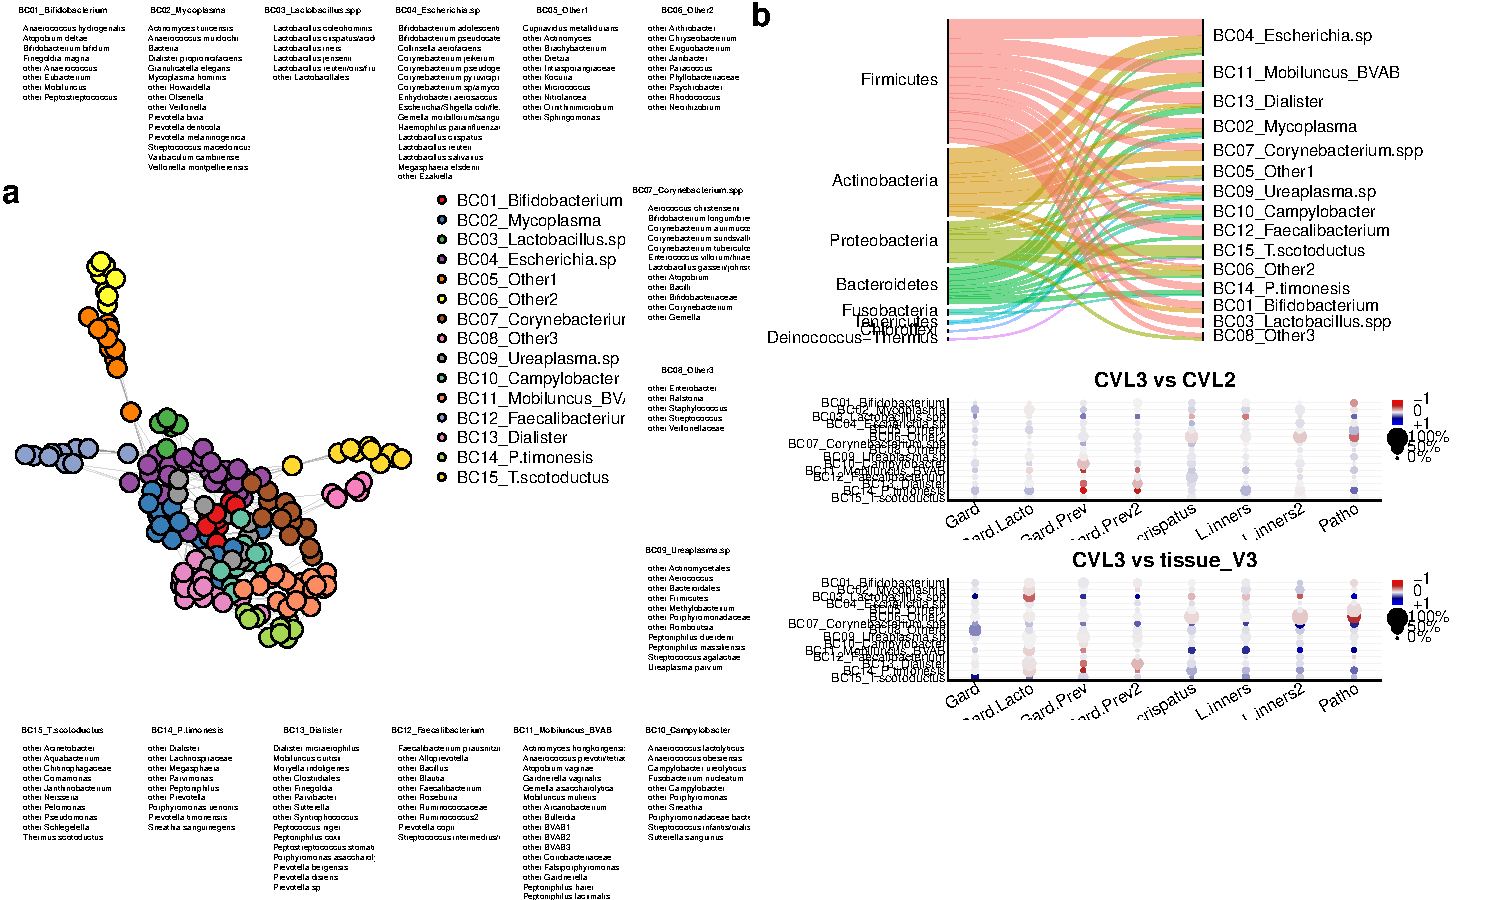
\includegraphics[width=1\linewidth]{manuscript_template_files/figure-latex/unnamed-chunk-6-1}
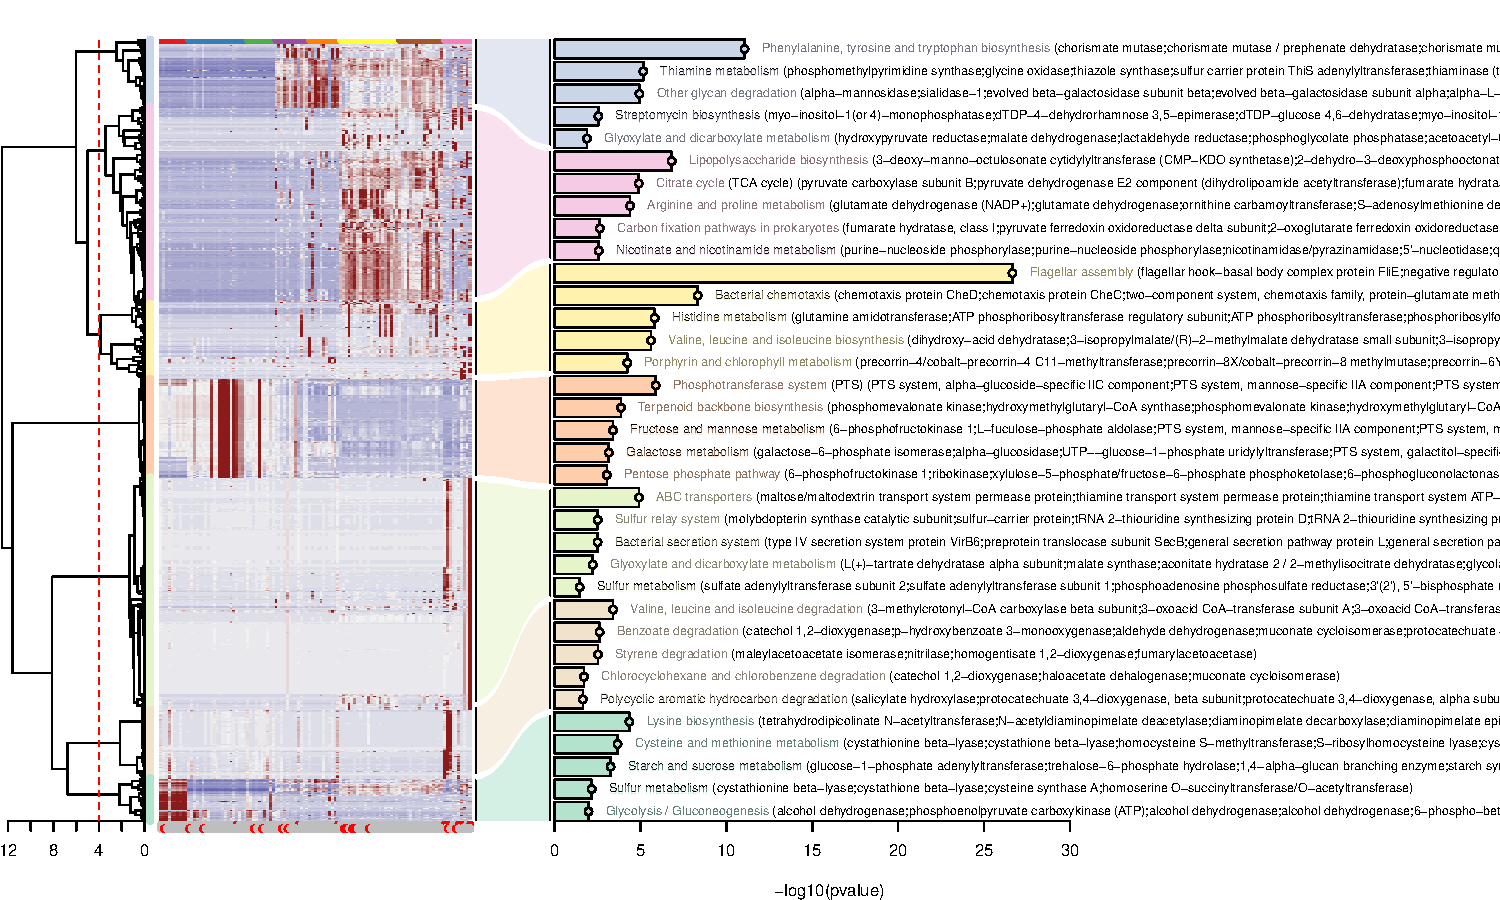
\includegraphics[width=1\linewidth]{manuscript_template_files/figure-latex/unnamed-chunk-6-2}
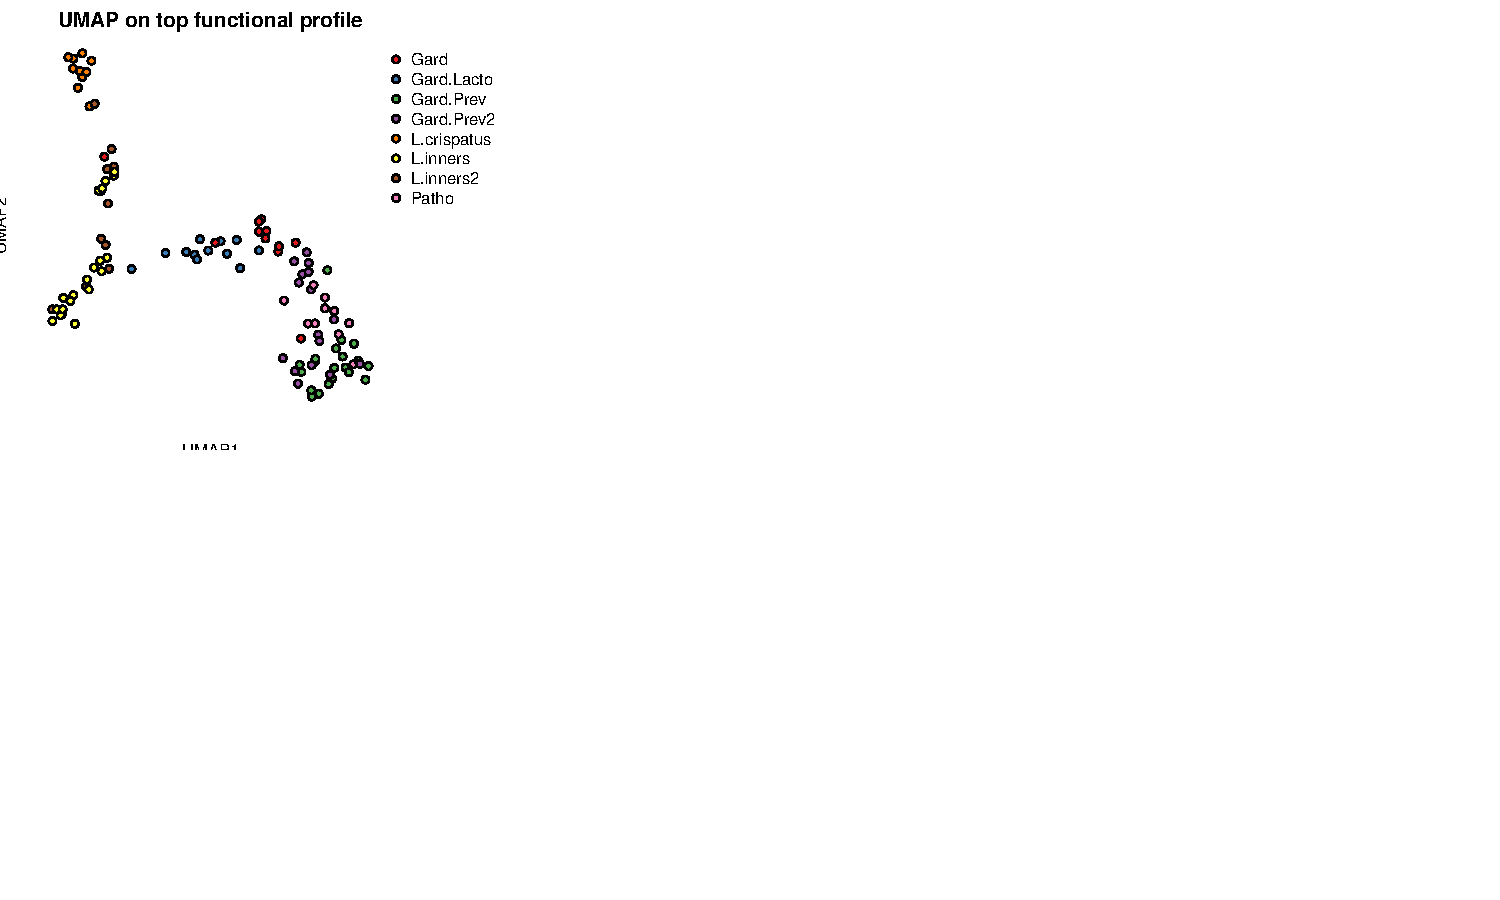
\includegraphics[width=1\linewidth]{manuscript_template_files/figure-latex/unnamed-chunk-6-3}

\textbf{Figure 2. Identification and characterization of vaginal bacterial communities.}
(\textbf{a}) Schematic representation of \#\#\#\#\#\#\#\#\#\# .
(\textbf{b}) Schematic representation of \#\#\#\#\#\#\#\#\#\# .
(\textbf{c}) Schematic representation of \#\#\#\#\#\#\#\#\#\# .
(\textbf{d}) Schematic representation of \#\#\#\#\#\#\#\#\#\# .

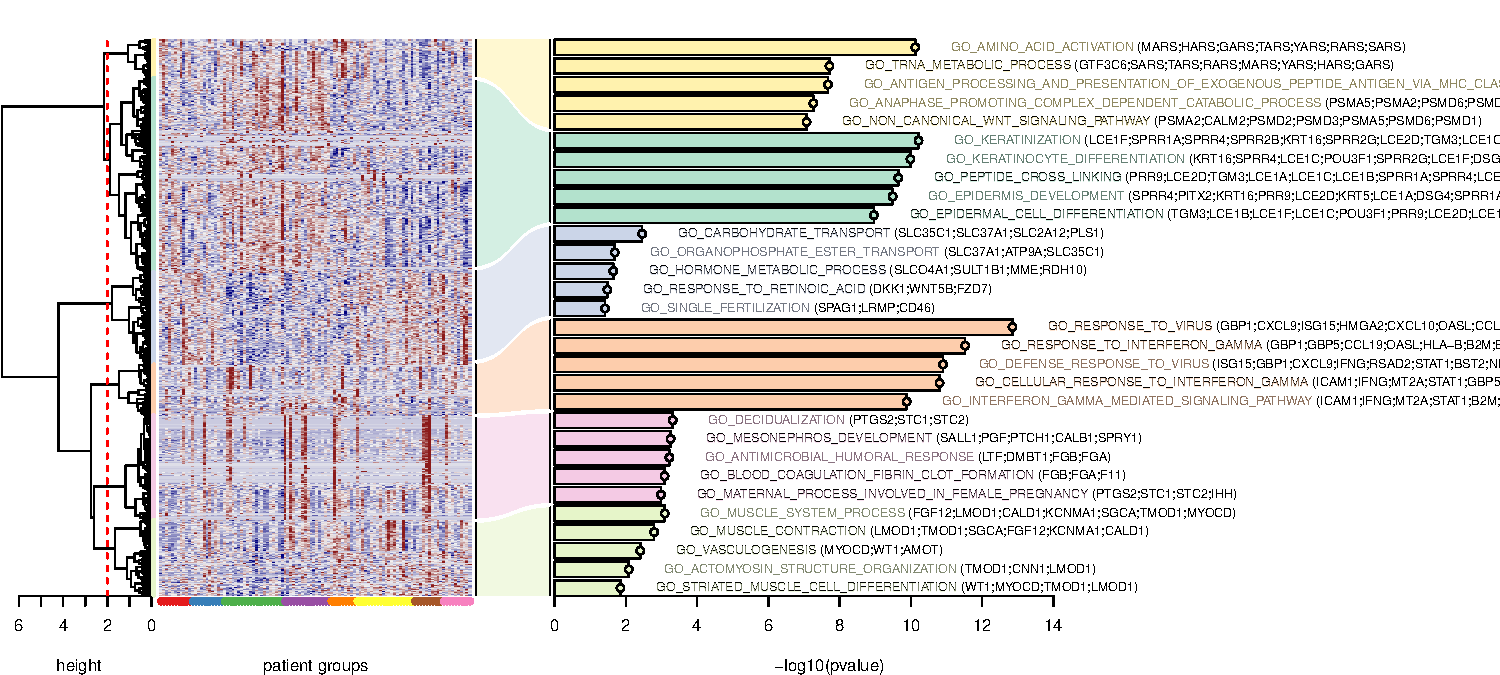
\includegraphics[width=1\linewidth]{manuscript_template_files/figure-latex/unnamed-chunk-7-1}

\clearpage

\hypertarget{figure-3}{%
\subsection{Figure 3}\label{figure-3}}

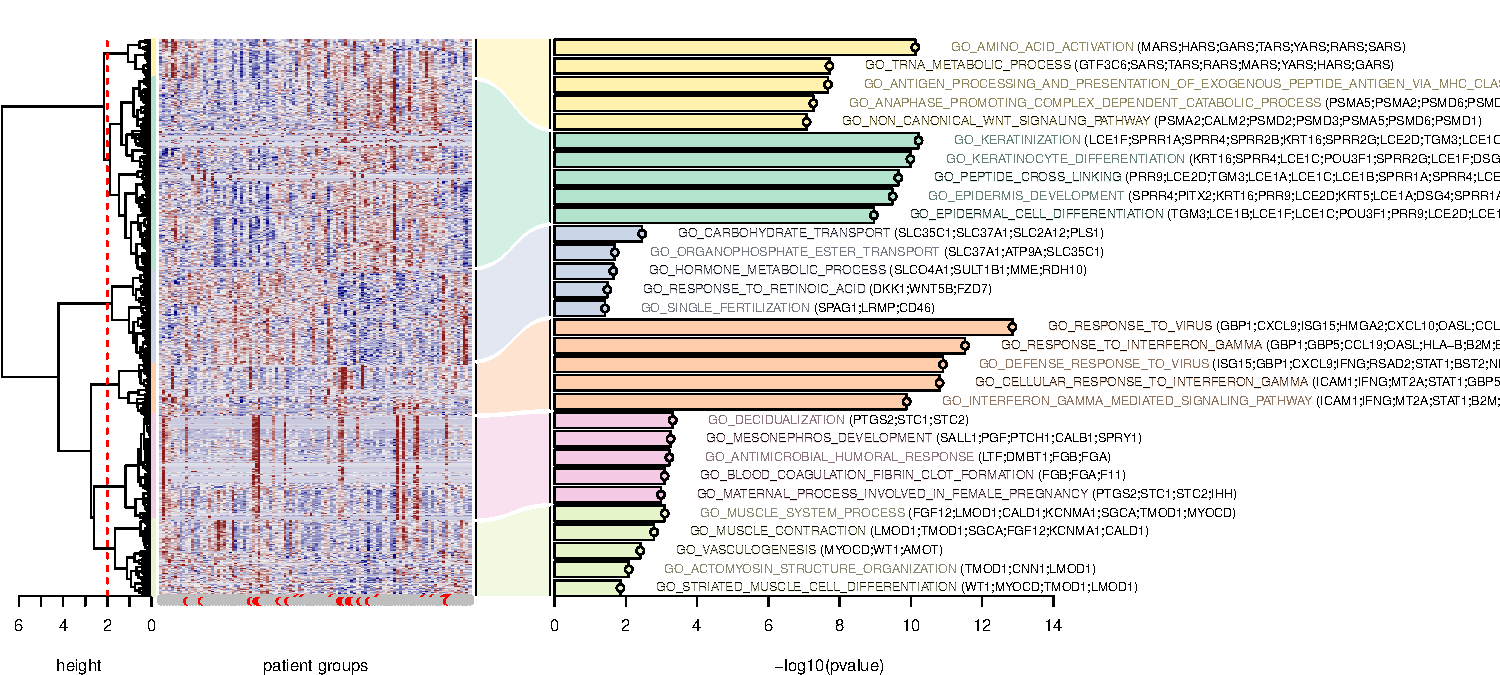
\includegraphics[width=1\linewidth]{manuscript_template_files/figure-latex/unnamed-chunk-8-1}
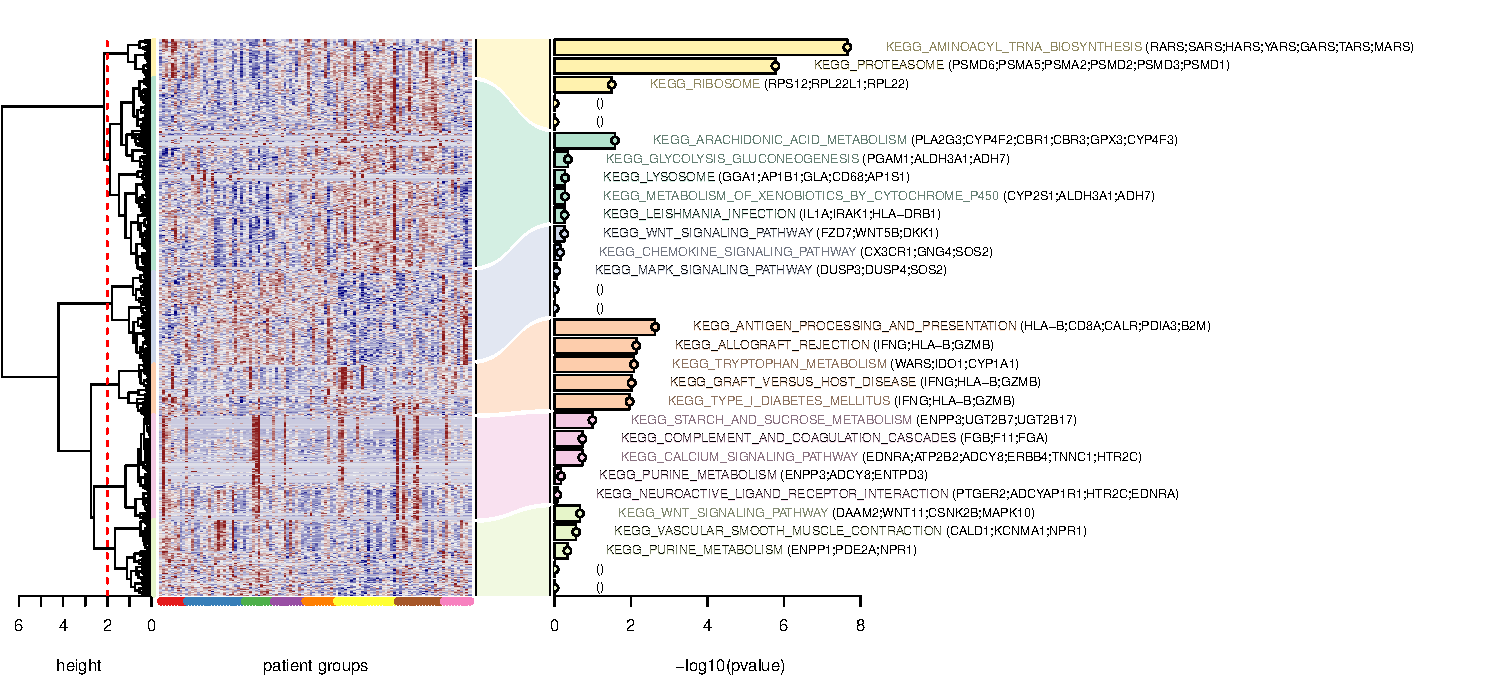
\includegraphics[width=1\linewidth]{manuscript_template_files/figure-latex/unnamed-chunk-8-2}
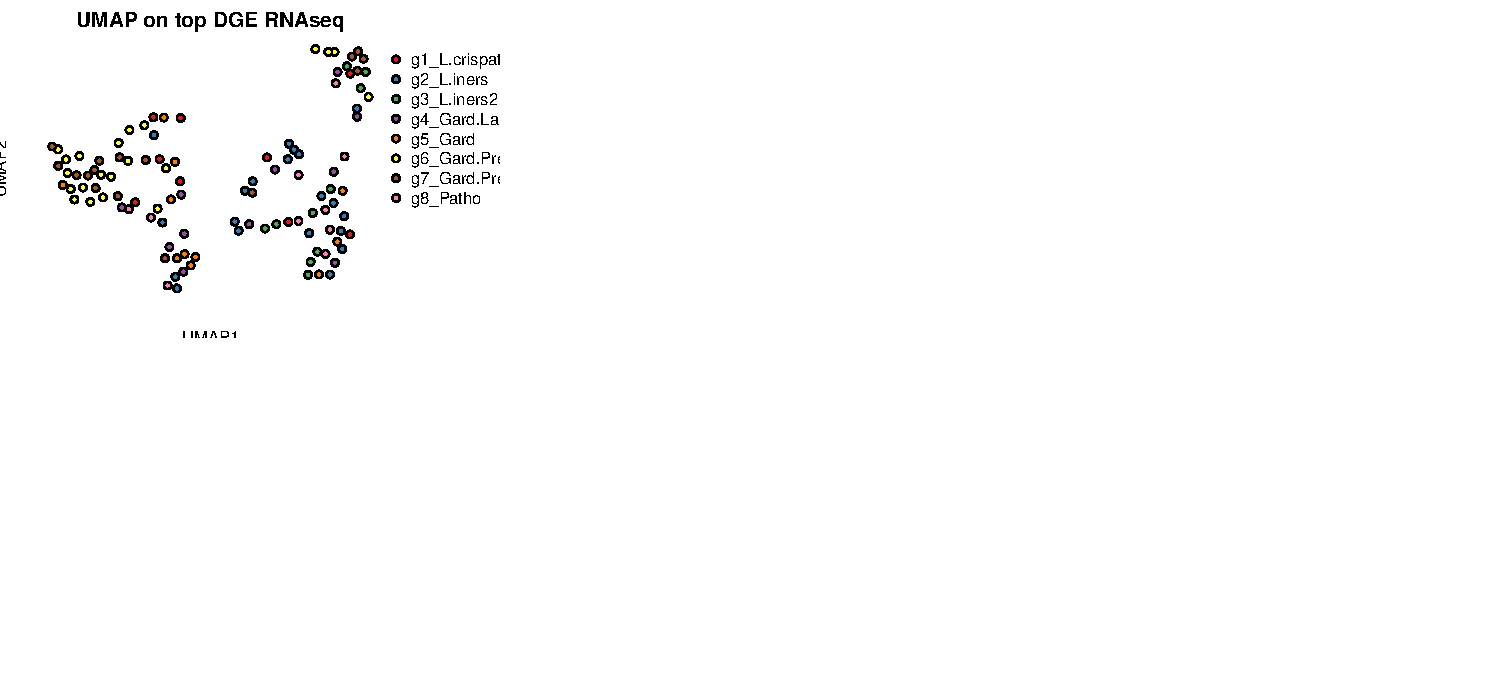
\includegraphics[width=1\linewidth]{manuscript_template_files/figure-latex/unnamed-chunk-8-3}
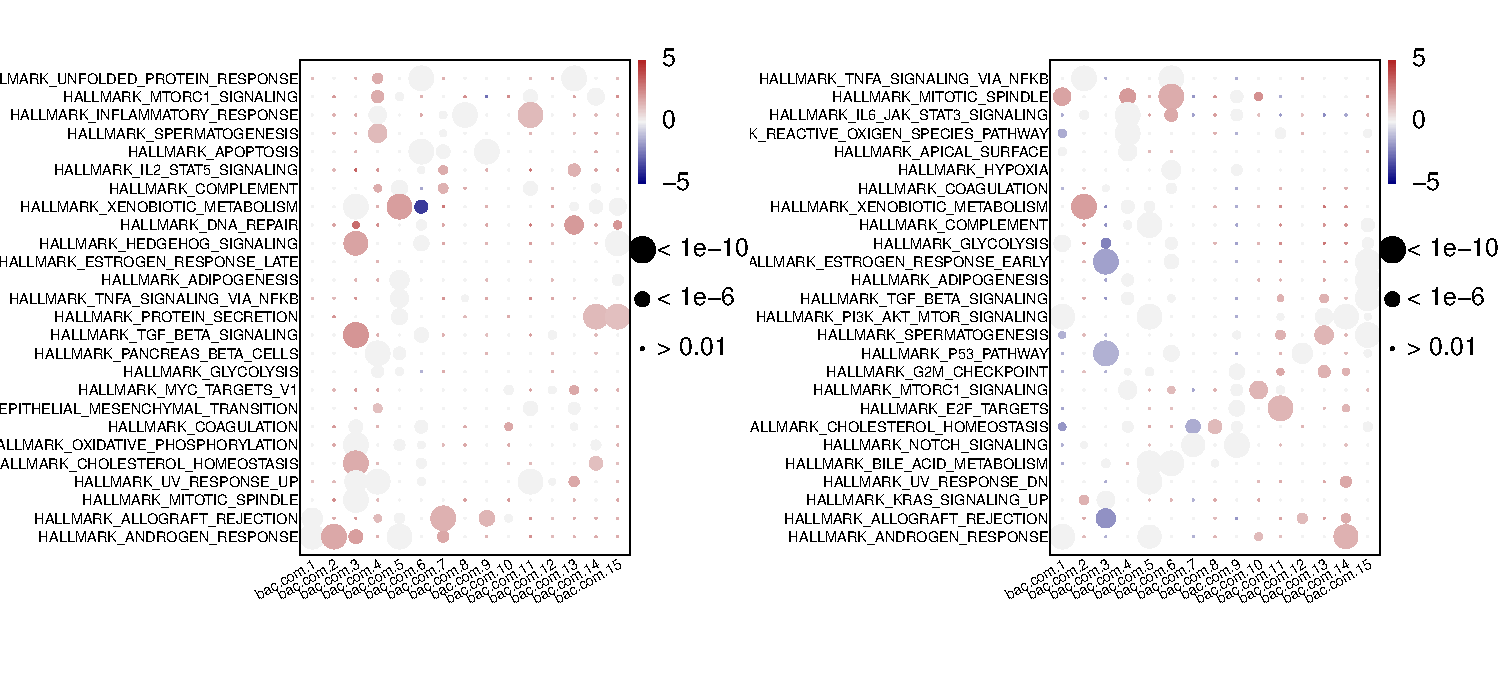
\includegraphics[width=1\linewidth]{manuscript_template_files/figure-latex/unnamed-chunk-8-4}

\textbf{Figure 1. Identification of patient groups.}
(\textbf{a}) Schematic representation of \#\#\#\#\#\#\#\#\#\# .
(\textbf{b}) Schematic representation of \#\#\#\#\#\#\#\#\#\# .
(\textbf{c}) Schematic representation of \#\#\#\#\#\#\#\#\#\# .
(\textbf{d}) Schematic representation of \#\#\#\#\#\#\#\#\#\# .

\clearpage

\hypertarget{figures-suppl}{%
\section{FIGURES (SUPPL)}\label{figures-suppl}}

\hypertarget{figure-s1}{%
\subsection{Figure S1}\label{figure-s1}}

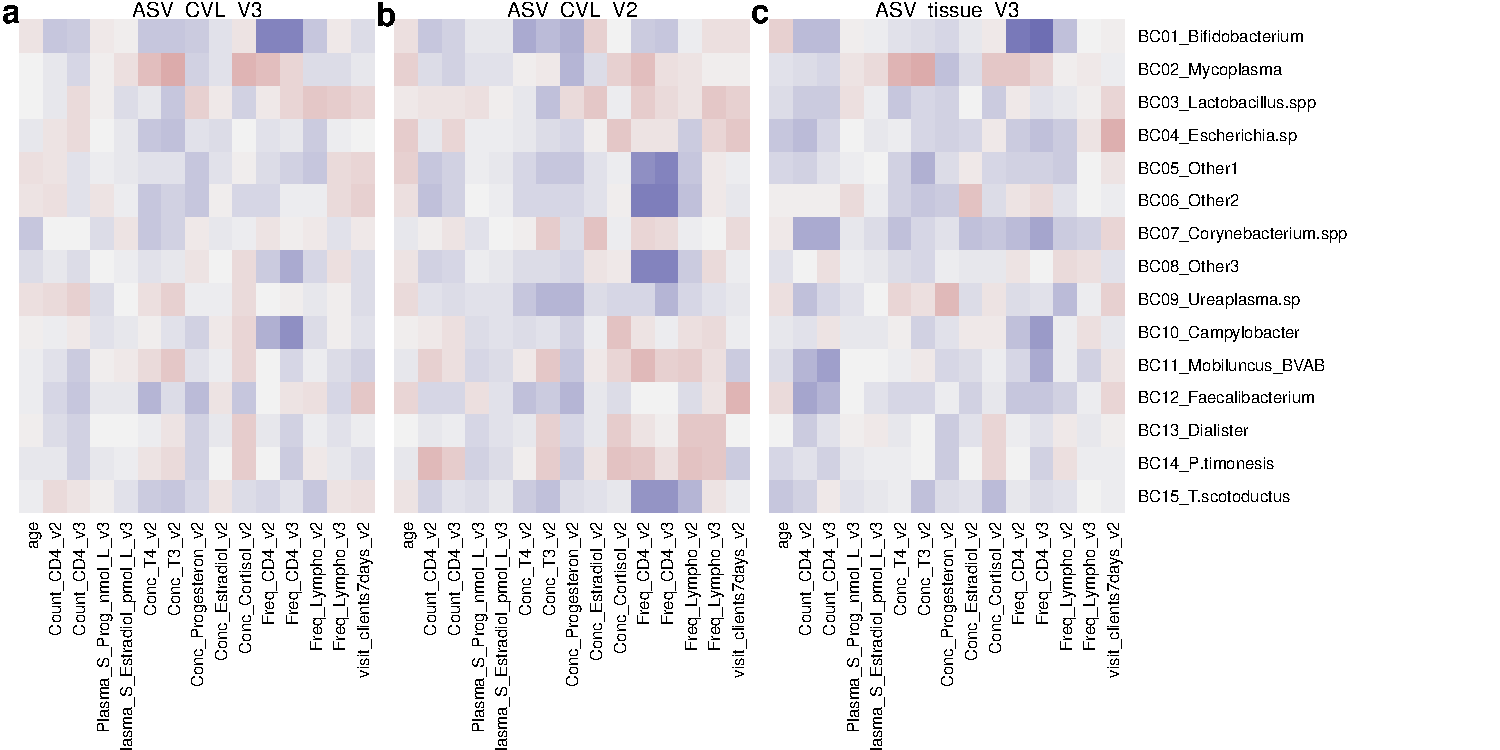
\includegraphics[width=1\linewidth]{manuscript_template_files/figure-latex/unnamed-chunk-9-1}

\clearpage

\hypertarget{figure-s2}{%
\subsection{Figure S2}\label{figure-s2}}

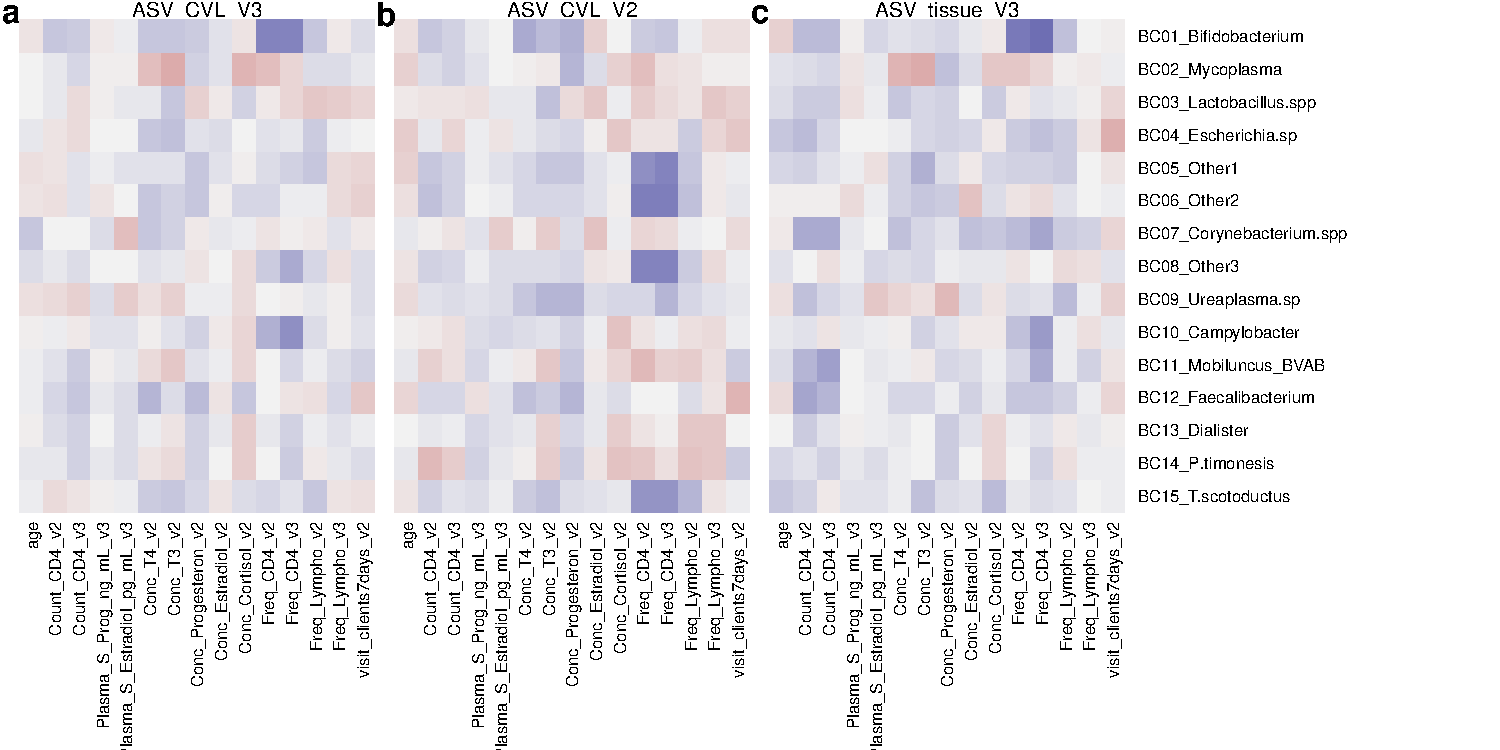
\includegraphics[width=1\linewidth]{manuscript_template_files/figure-latex/unnamed-chunk-10-1}

\clearpage

\hypertarget{figure-s2-v2}{%
\subsection{Figure S2 v2}\label{figure-s2-v2}}

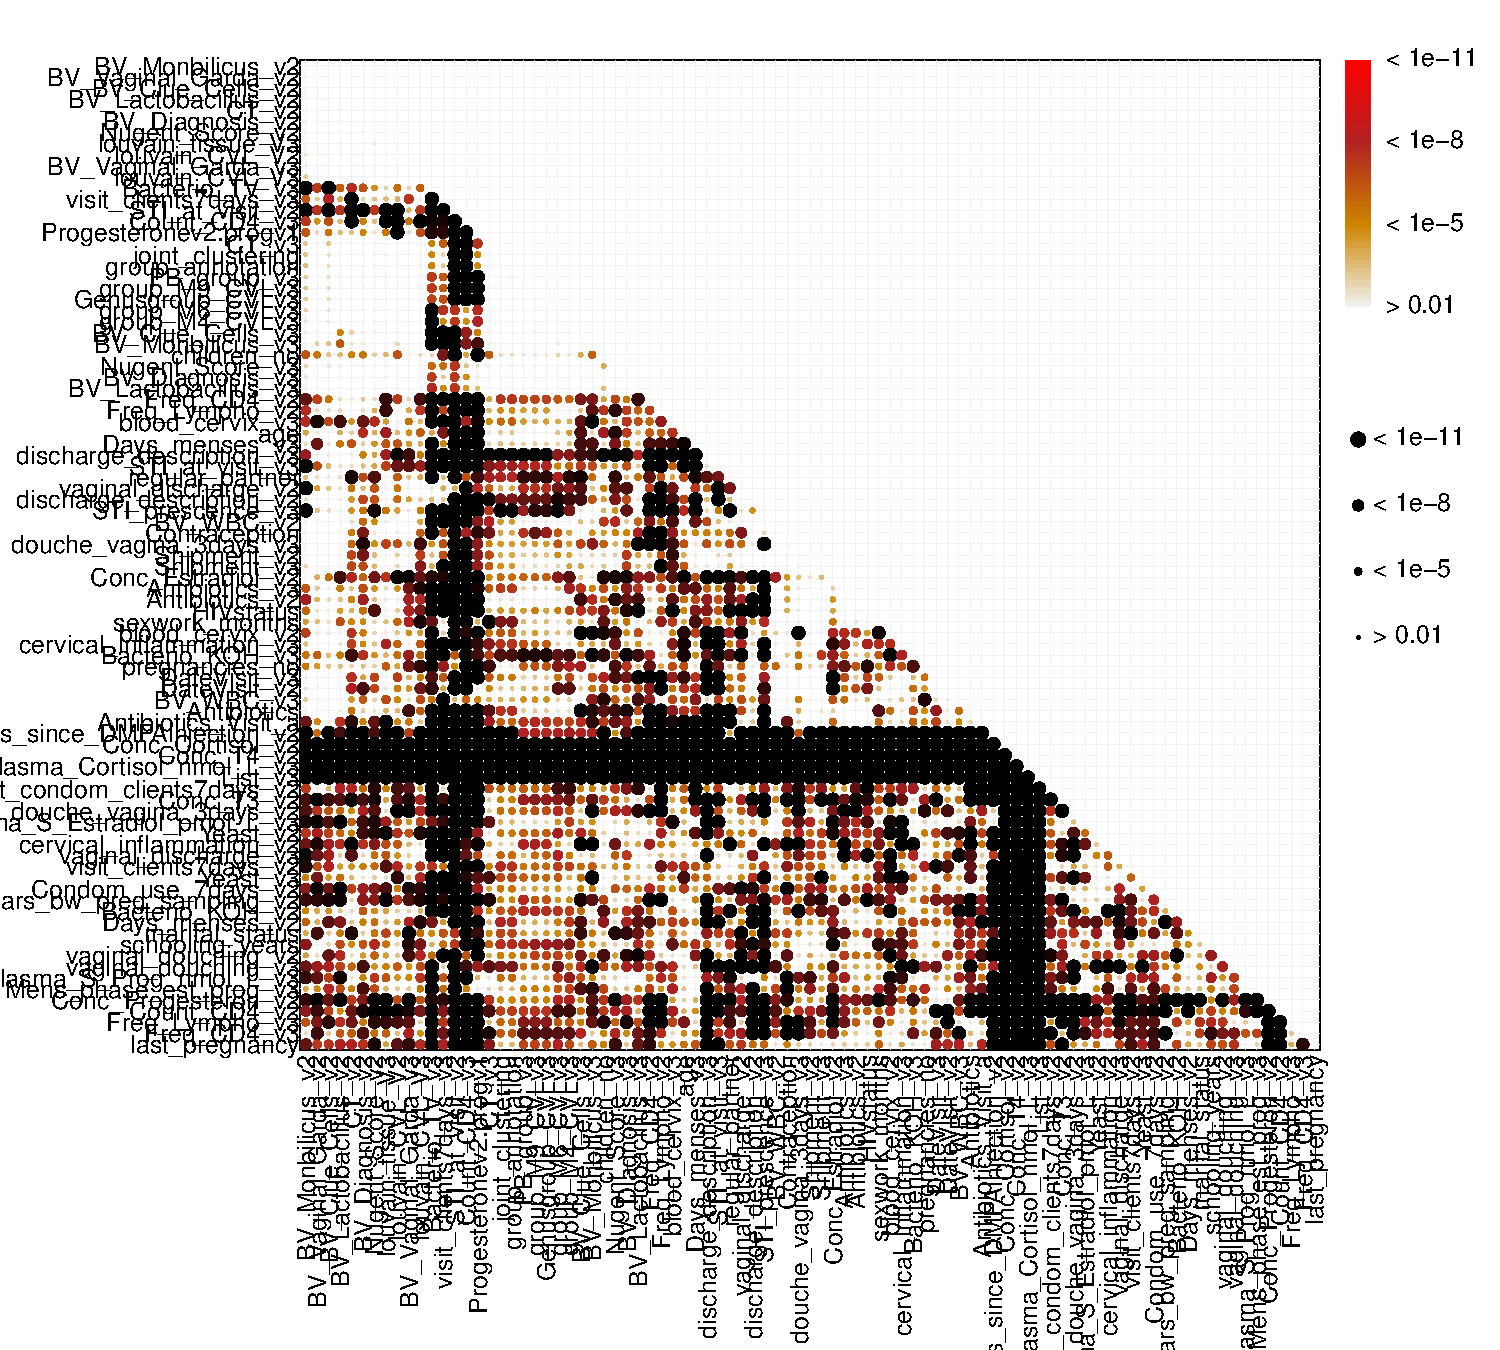
\includegraphics[width=1\linewidth]{manuscript_template_files/figure-latex/unnamed-chunk-11-1}

\clearpage

\hypertarget{figure-s2-v3}{%
\subsection{Figure S2 v3}\label{figure-s2-v3}}

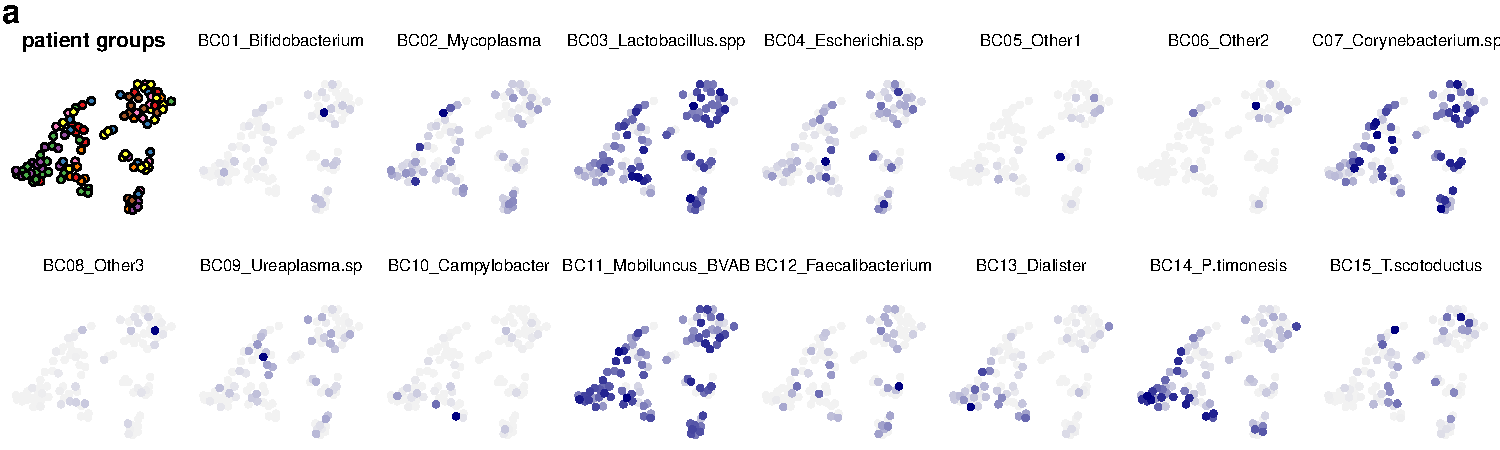
\includegraphics[width=1\linewidth]{manuscript_template_files/figure-latex/unnamed-chunk-12-1}

\clearpage

\hypertarget{figure-s3}{%
\subsection{Figure S3}\label{figure-s3}}

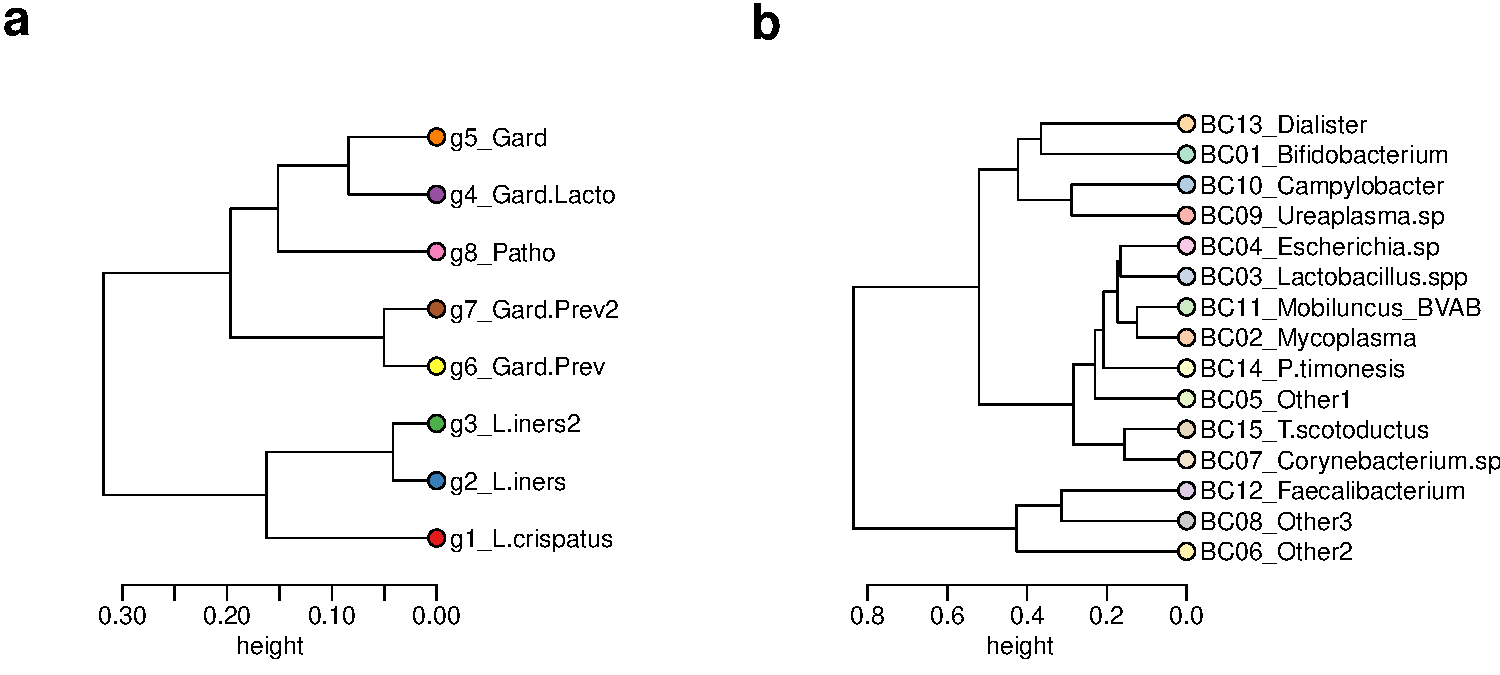
\includegraphics[width=1\linewidth]{manuscript_template_files/figure-latex/unnamed-chunk-13-1}

\clearpage

\hypertarget{figure-s4}{%
\subsection{Figure S4}\label{figure-s4}}

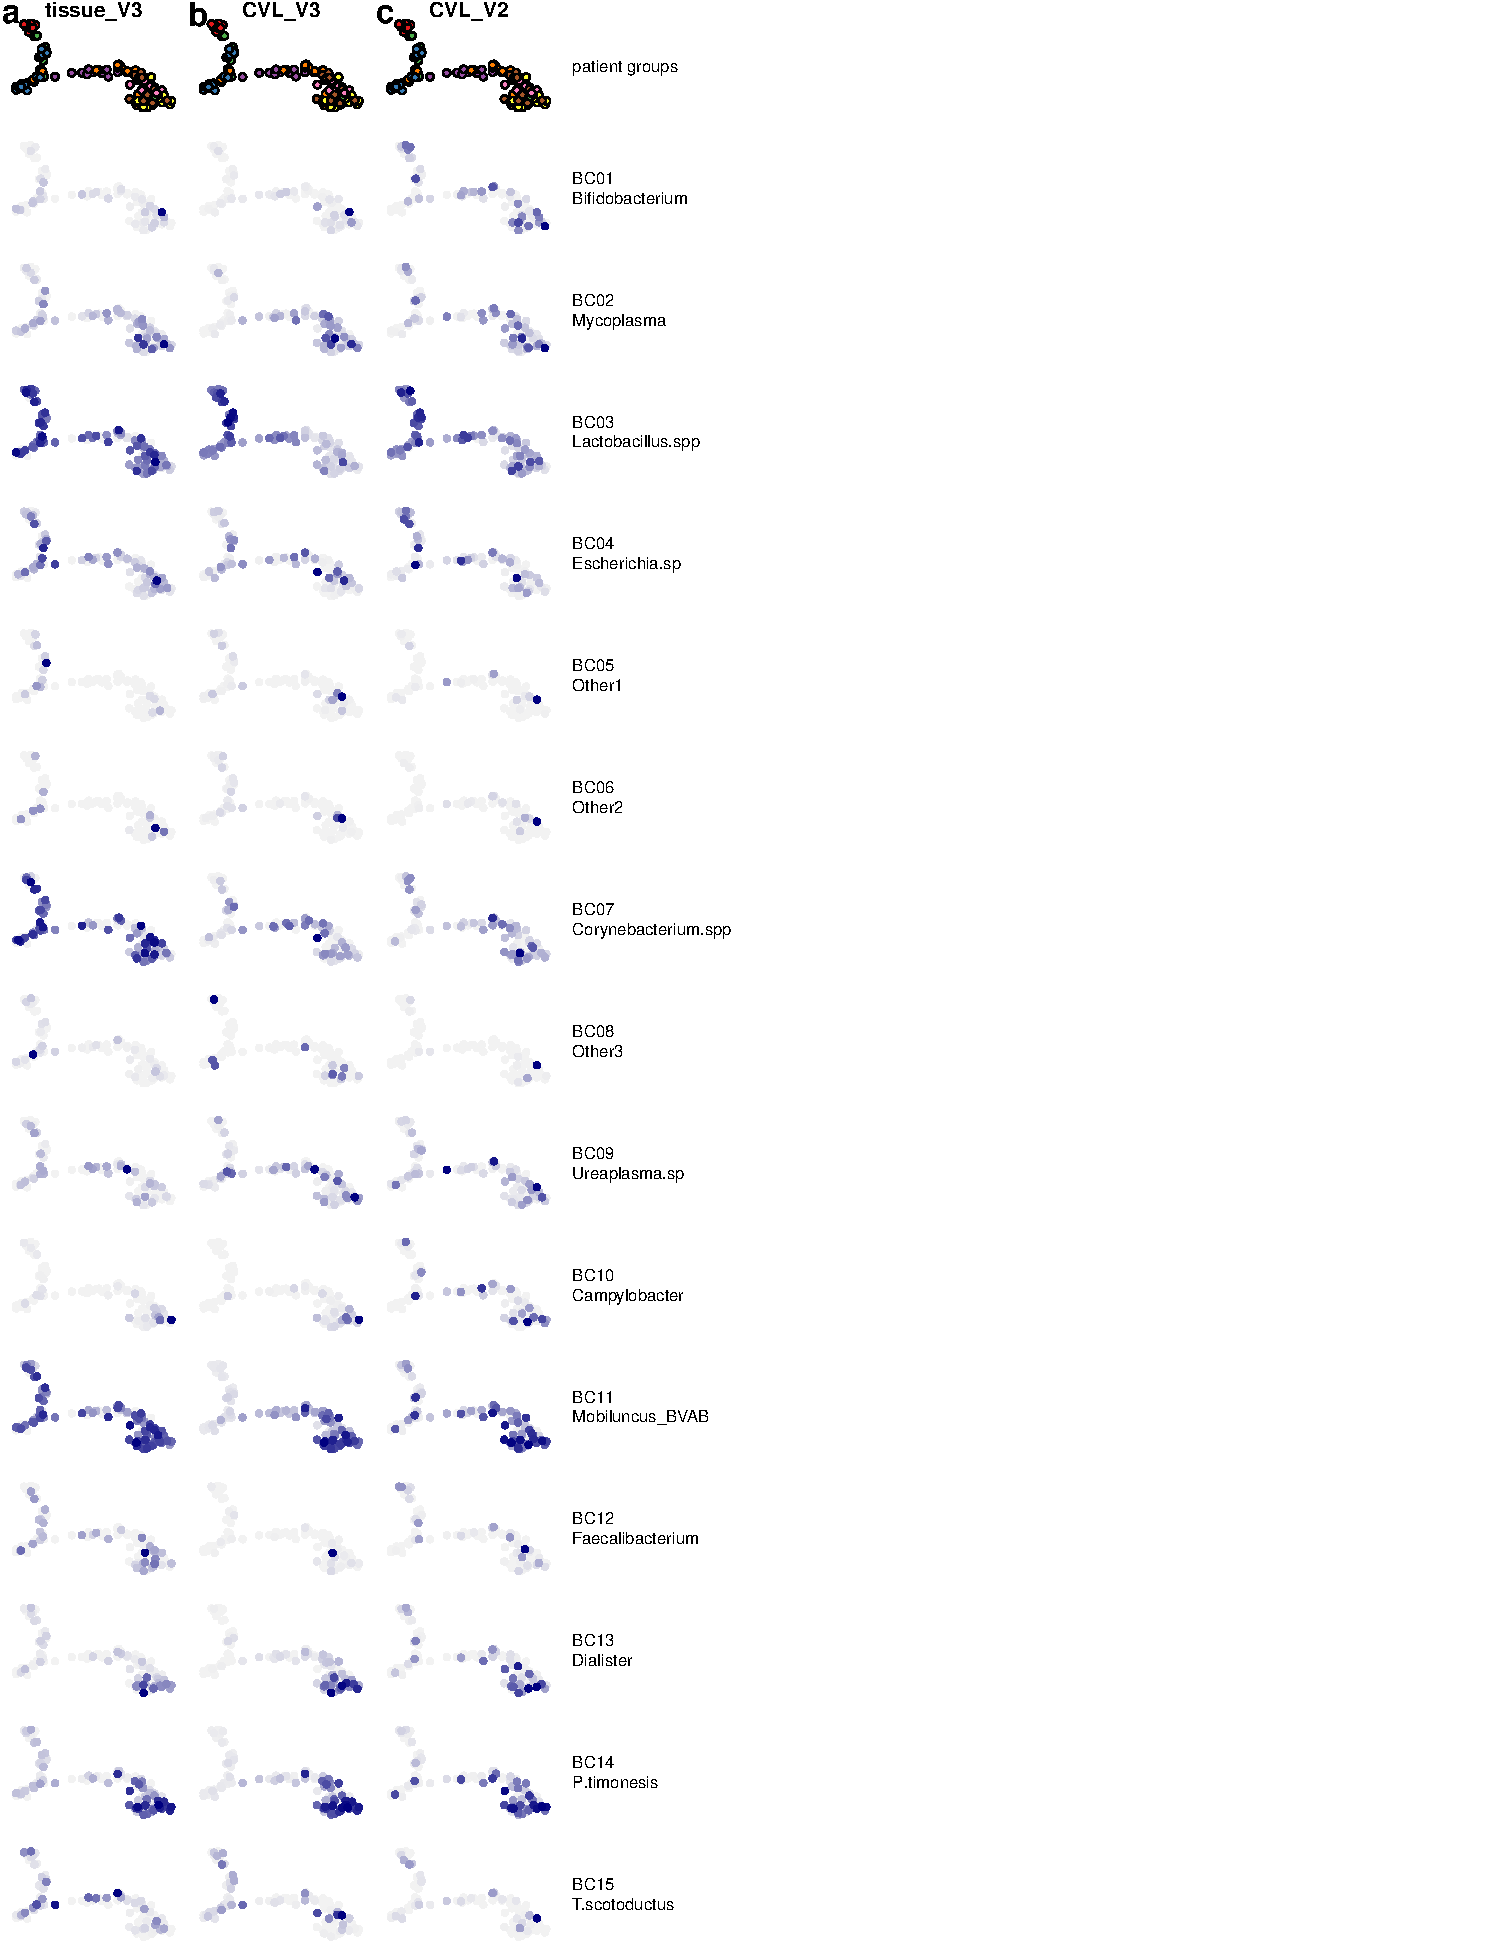
\includegraphics[width=1\linewidth]{manuscript_template_files/figure-latex/unnamed-chunk-14-1}

\clearpage

\hypertarget{figure-s5}{%
\subsection{Figure S5}\label{figure-s5}}

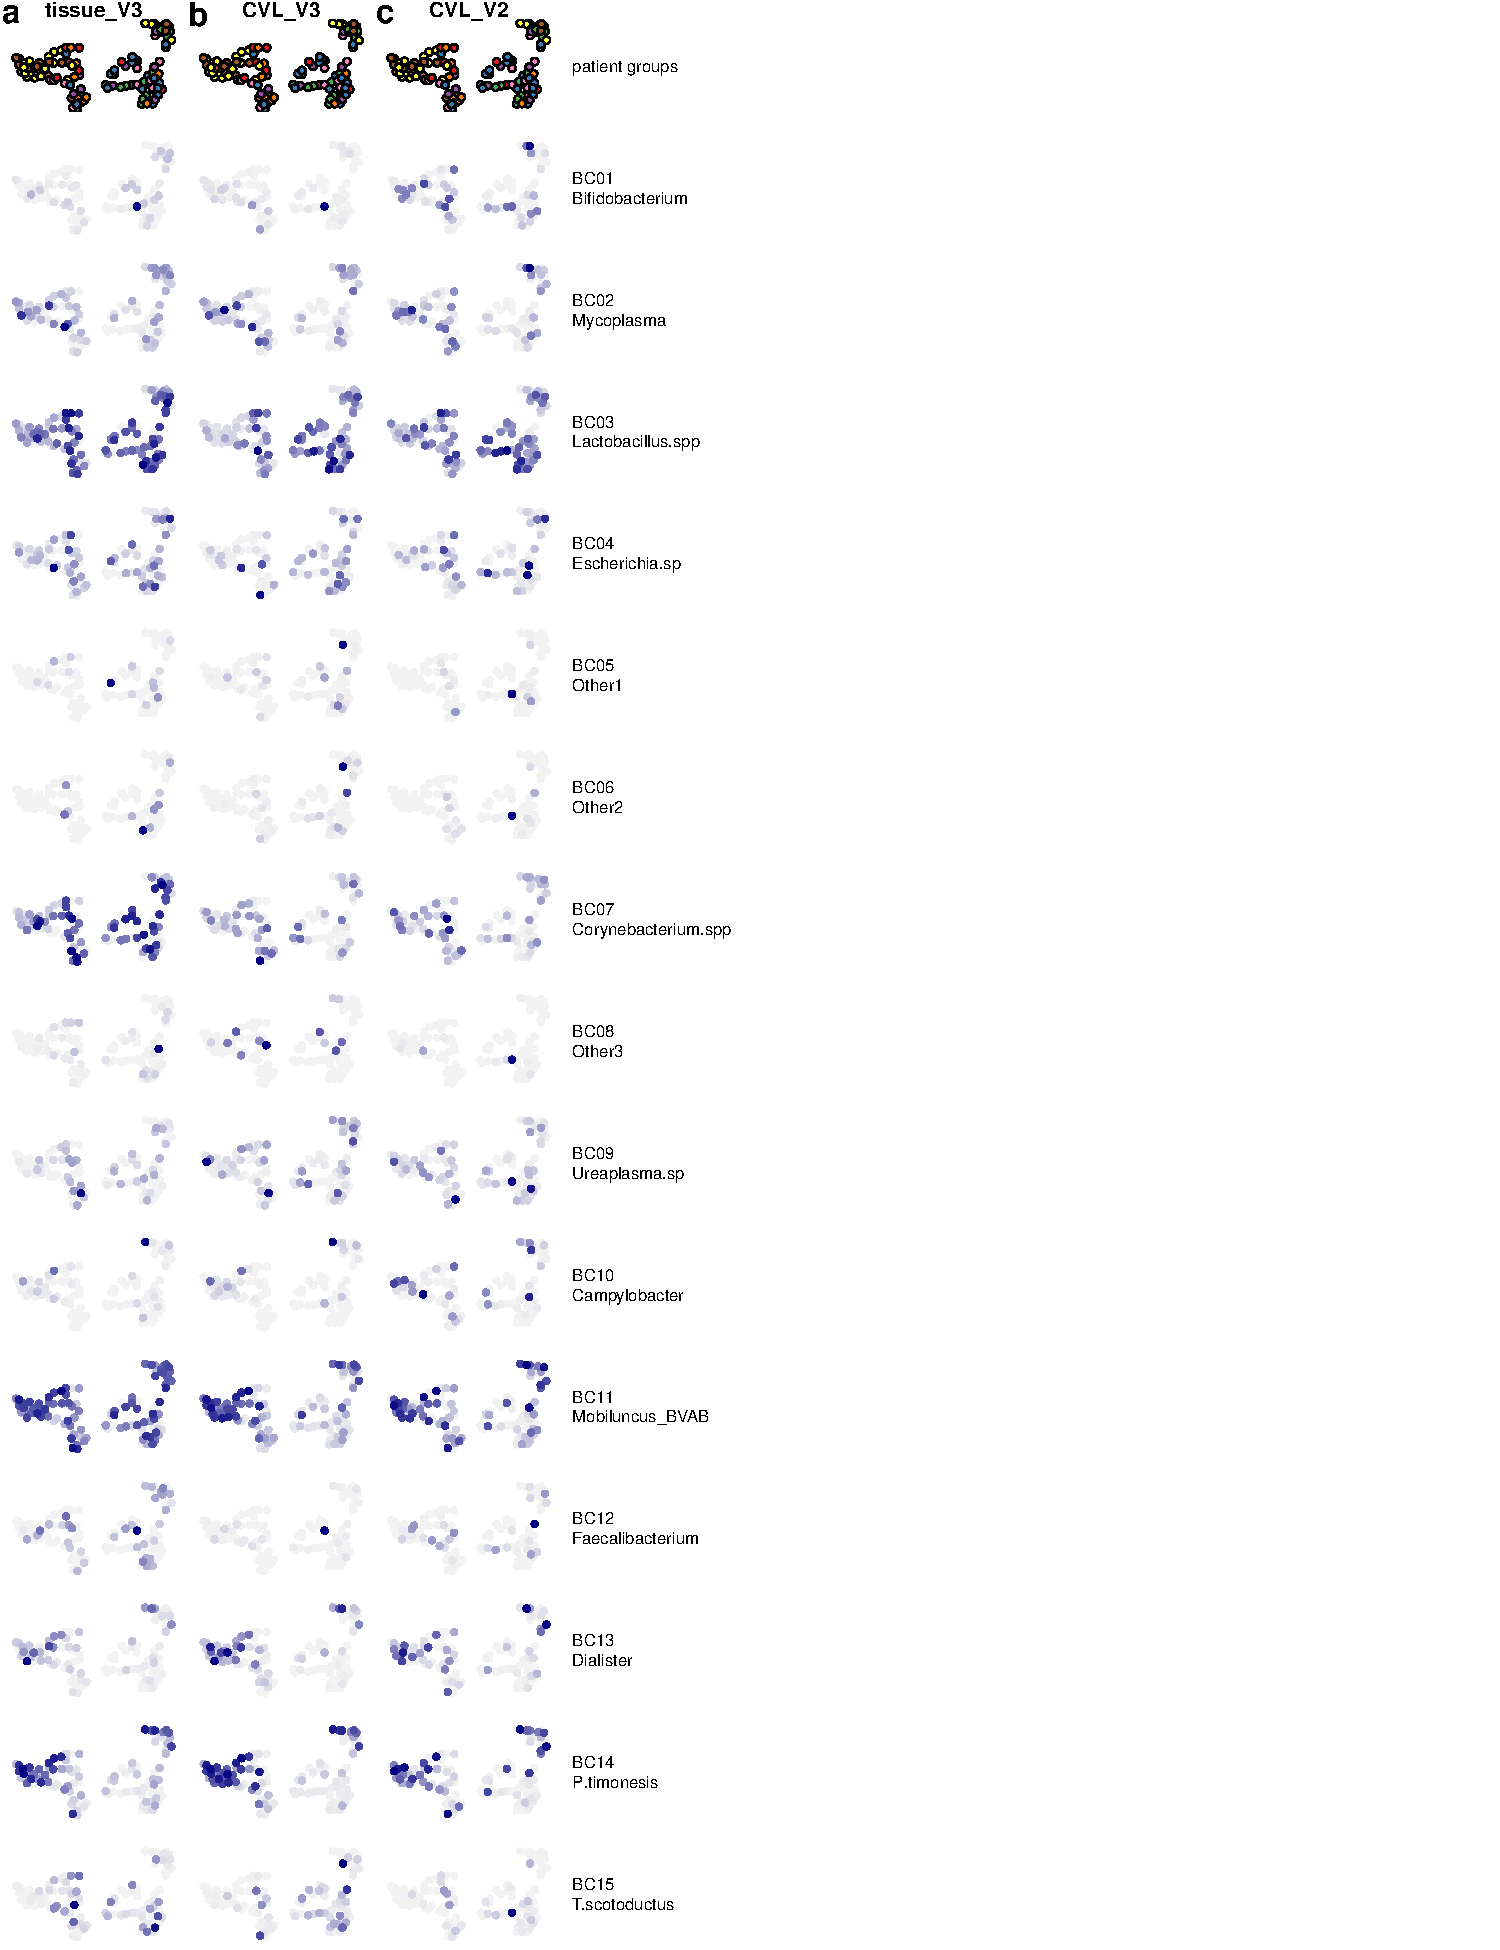
\includegraphics[width=1\linewidth]{manuscript_template_files/figure-latex/unnamed-chunk-15-1}

\clearpage

\hypertarget{figure-s6}{%
\subsection{Figure S6}\label{figure-s6}}

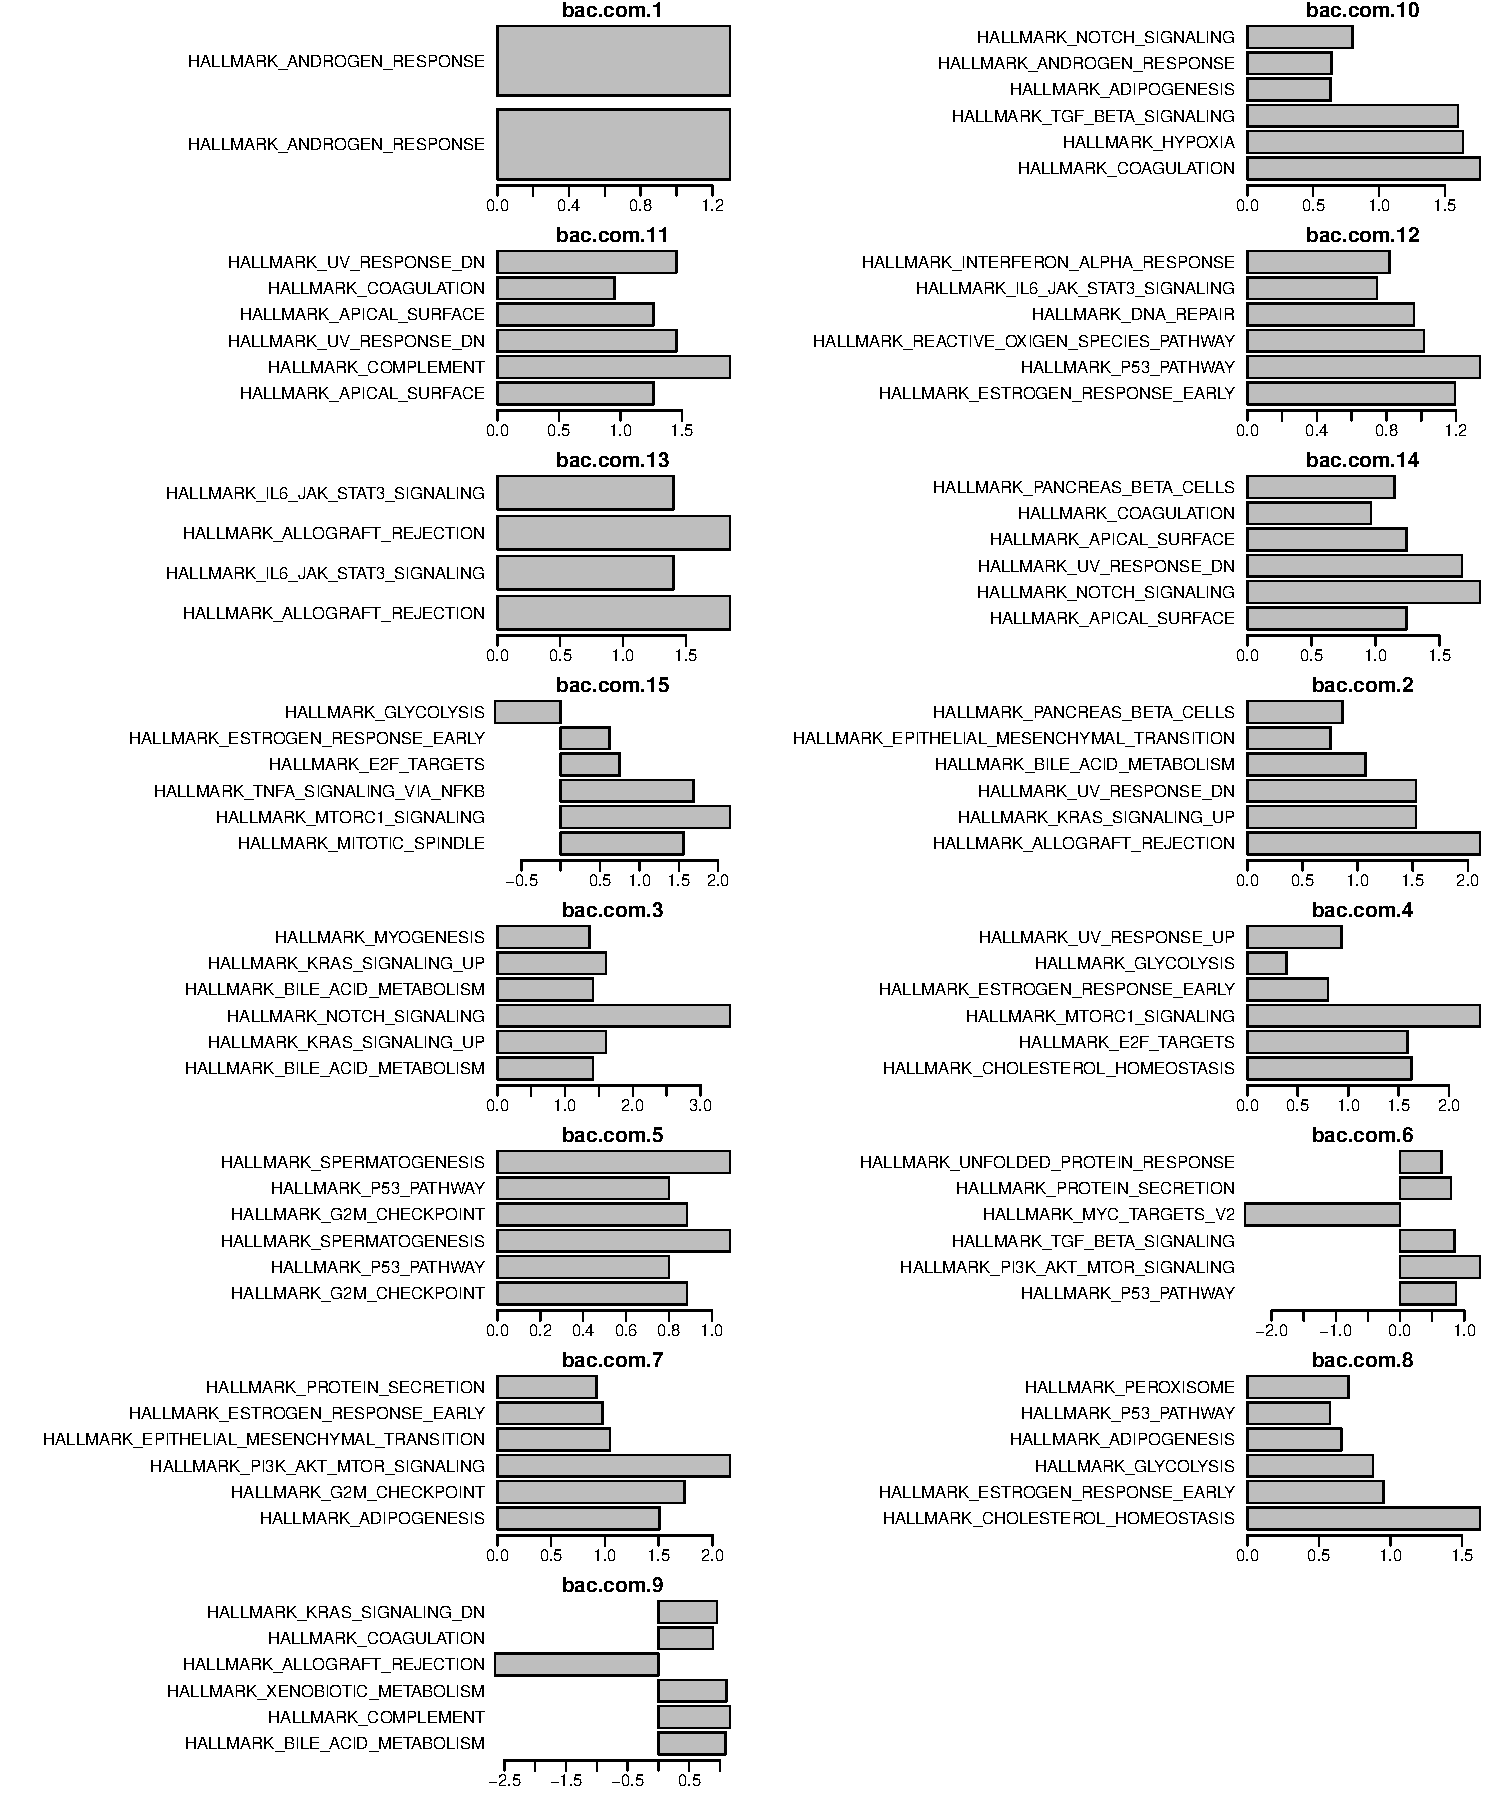
\includegraphics[width=1\linewidth]{manuscript_template_files/figure-latex/unnamed-chunk-16-1}

\clearpage

\hypertarget{figure-s7}{%
\subsection{Figure S7}\label{figure-s7}}

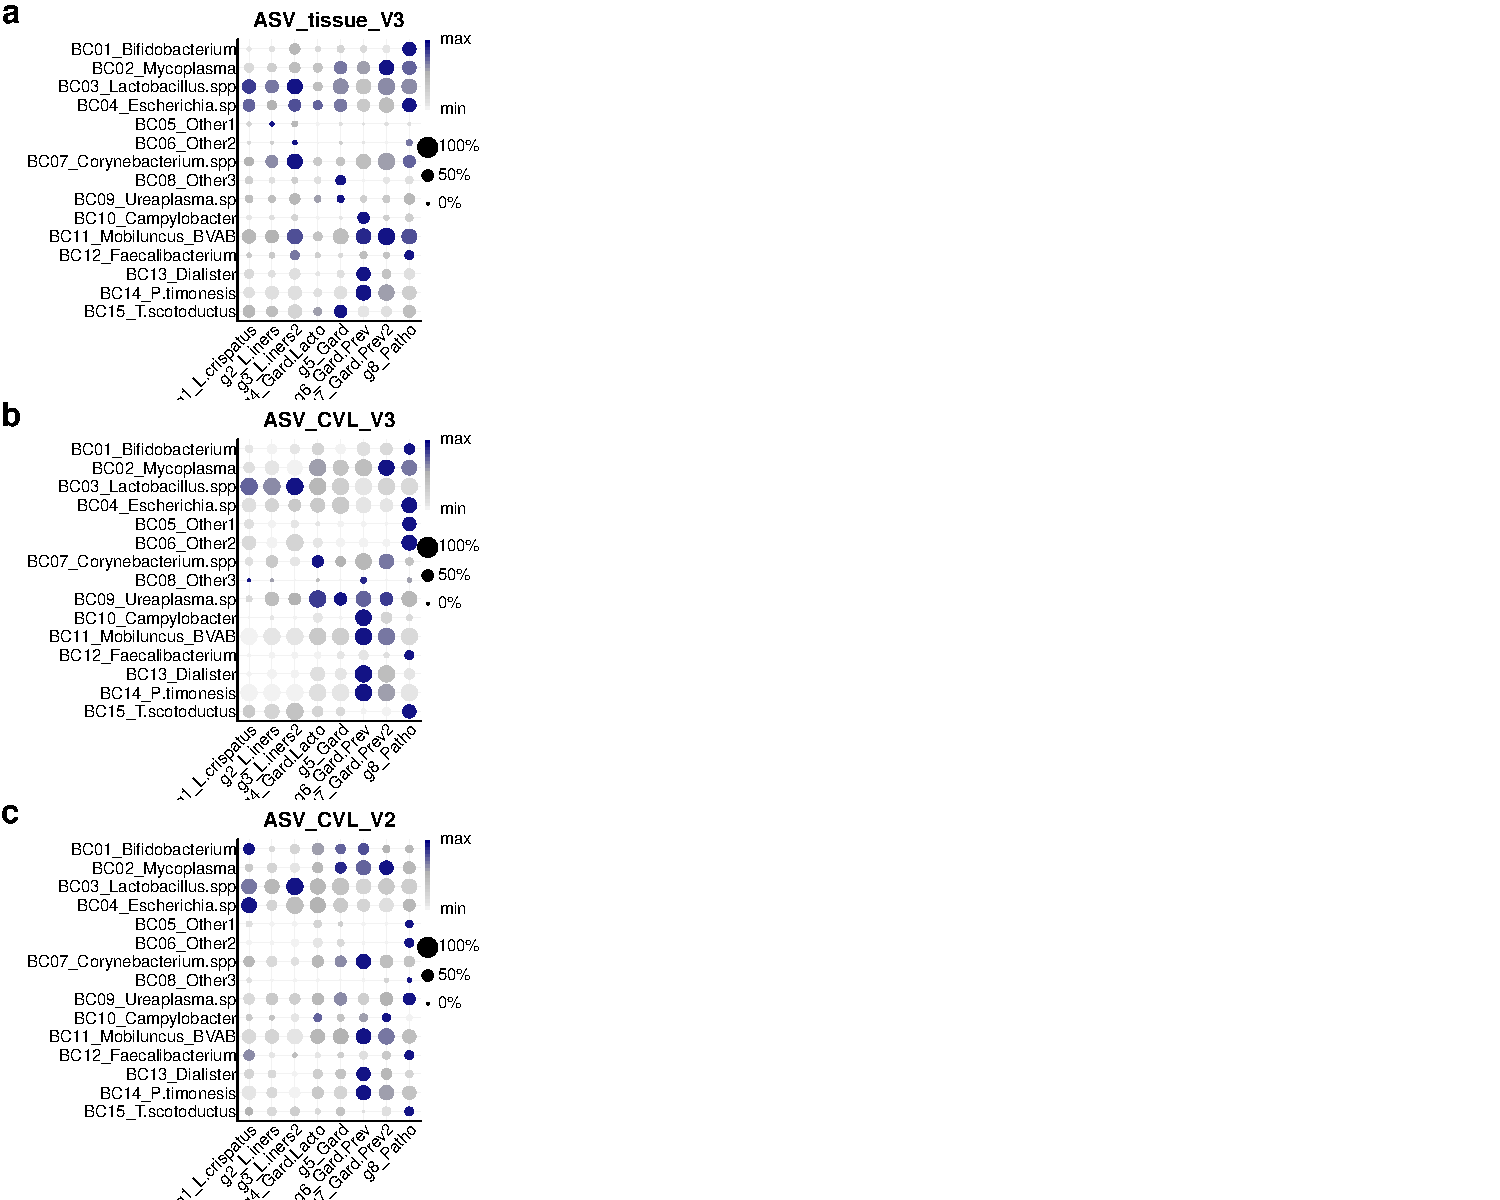
\includegraphics[width=1\linewidth]{manuscript_template_files/figure-latex/unnamed-chunk-17-1}

\clearpage

\hypertarget{figure-s8}{%
\subsection{Figure S8}\label{figure-s8}}

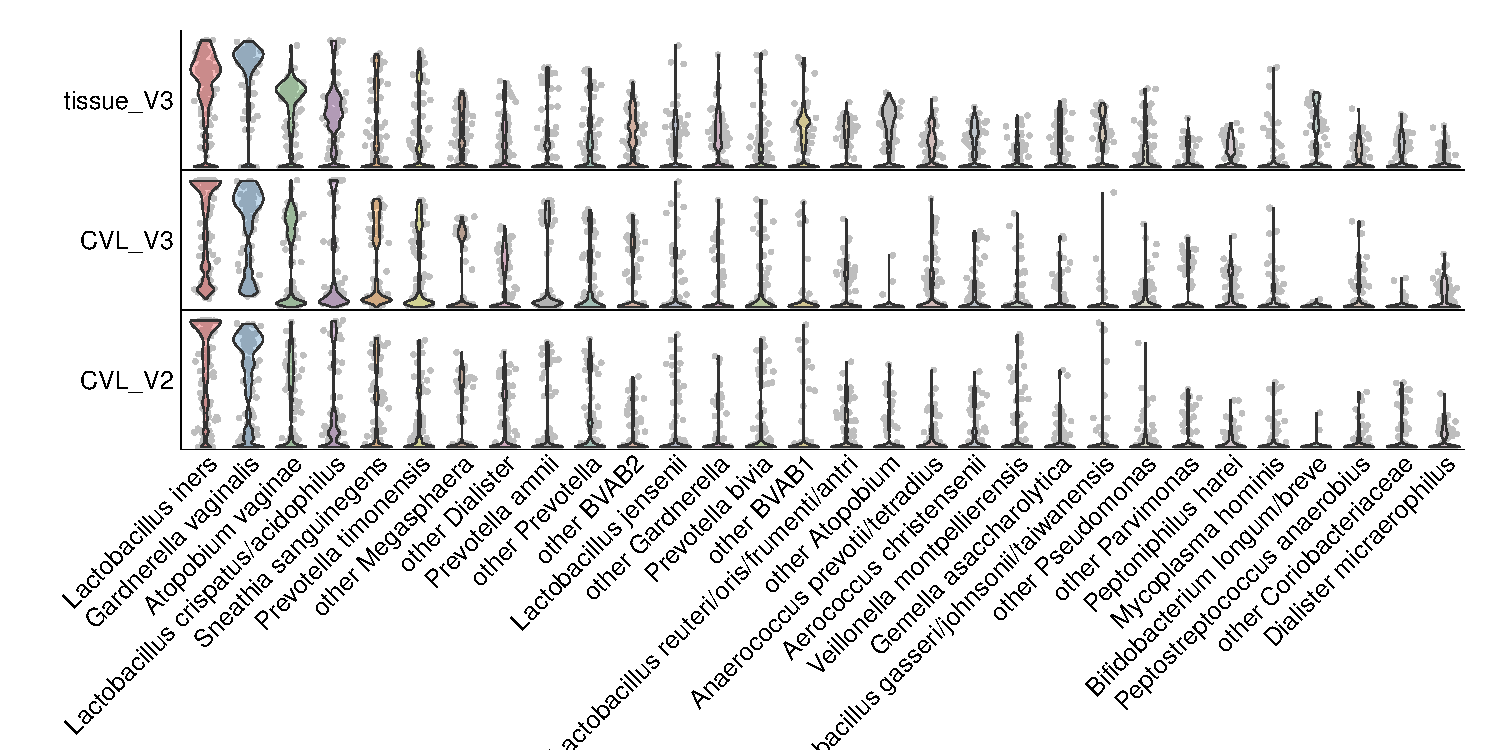
\includegraphics[width=1\linewidth]{manuscript_template_files/figure-latex/unnamed-chunk-18-1}

\clearpage

\hypertarget{figure-s9}{%
\subsection{Figure S9}\label{figure-s9}}

\clearpage

\hypertarget{figure-s10}{%
\subsection{Figure S10}\label{figure-s10}}

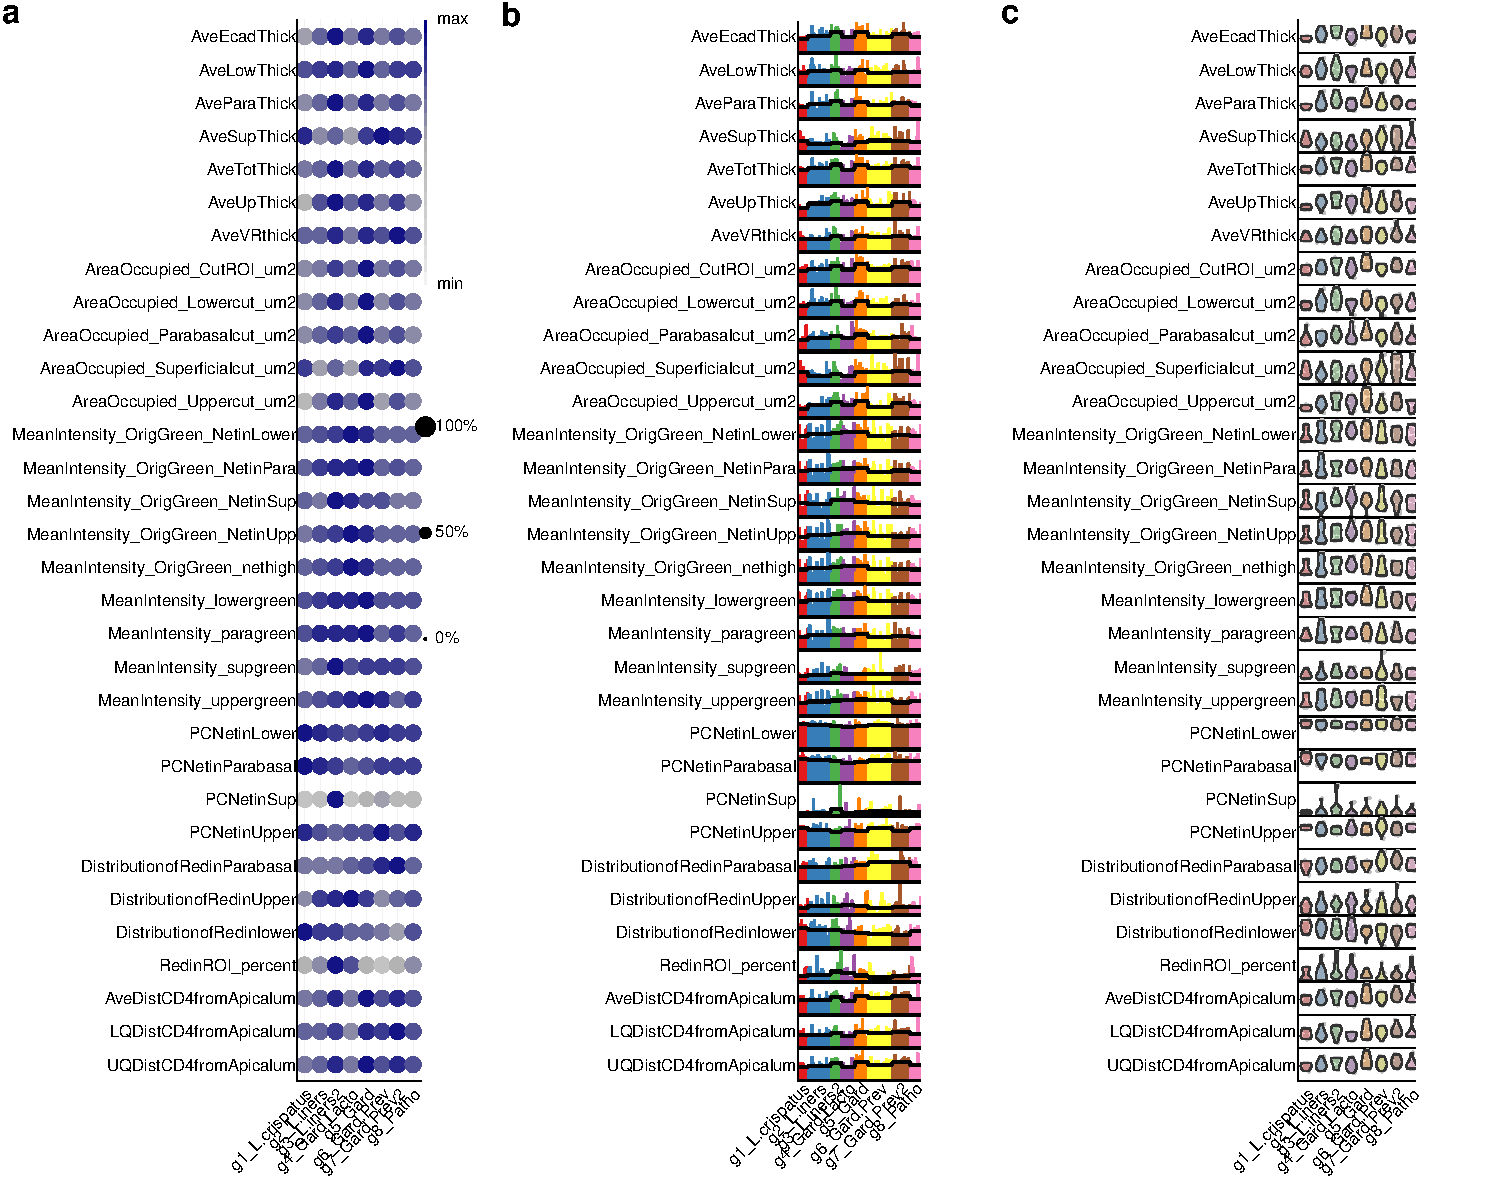
\includegraphics[width=1\linewidth]{manuscript_template_files/figure-latex/unnamed-chunk-20-1}
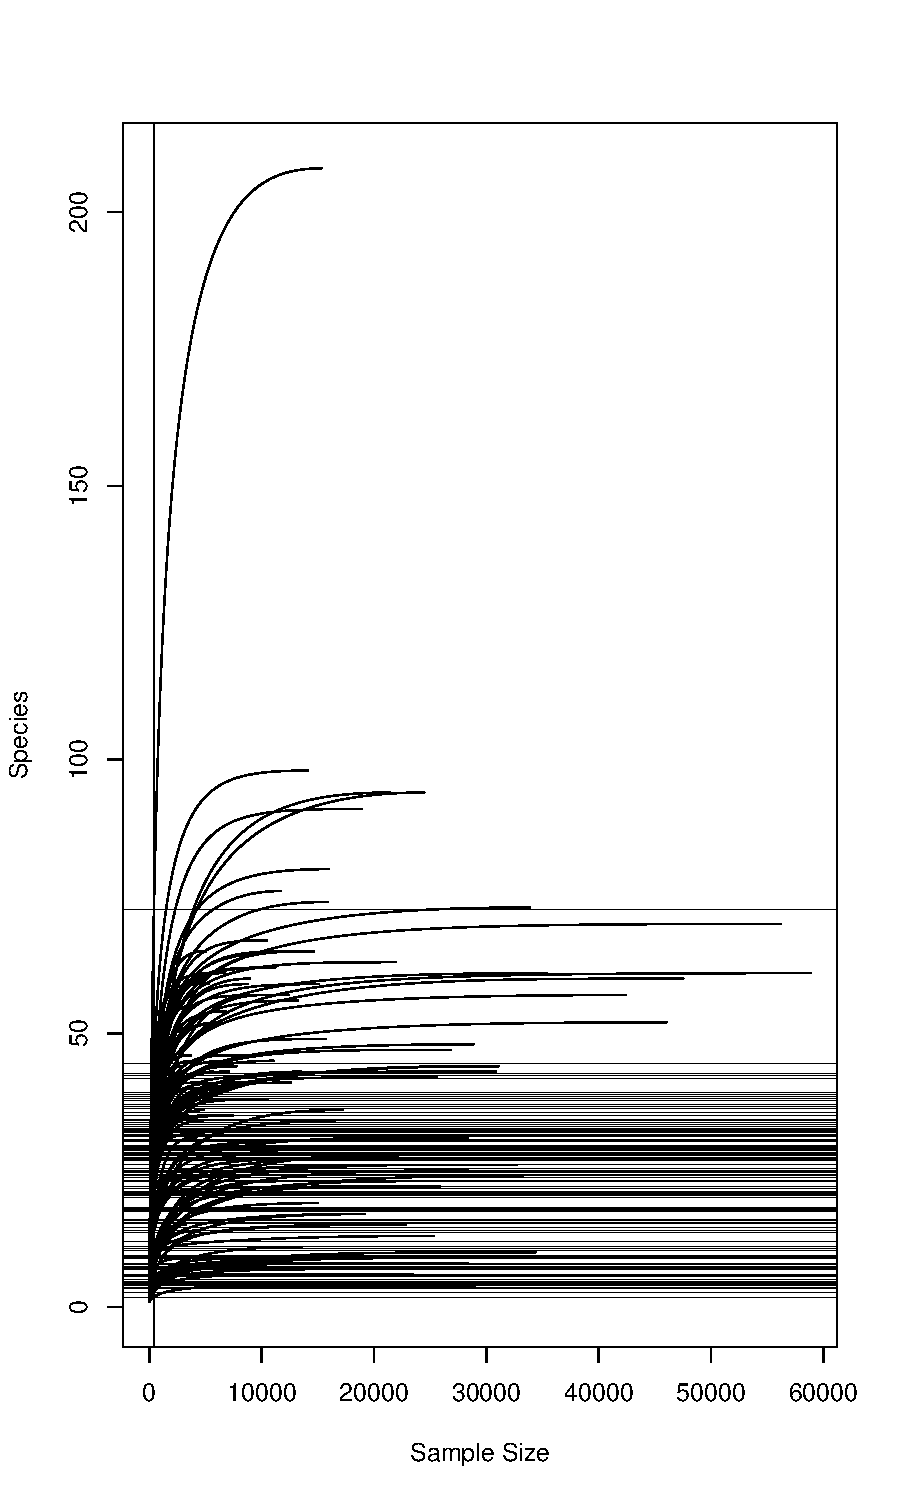
\includegraphics[width=1\linewidth]{manuscript_template_files/figure-latex/unnamed-chunk-20-2}
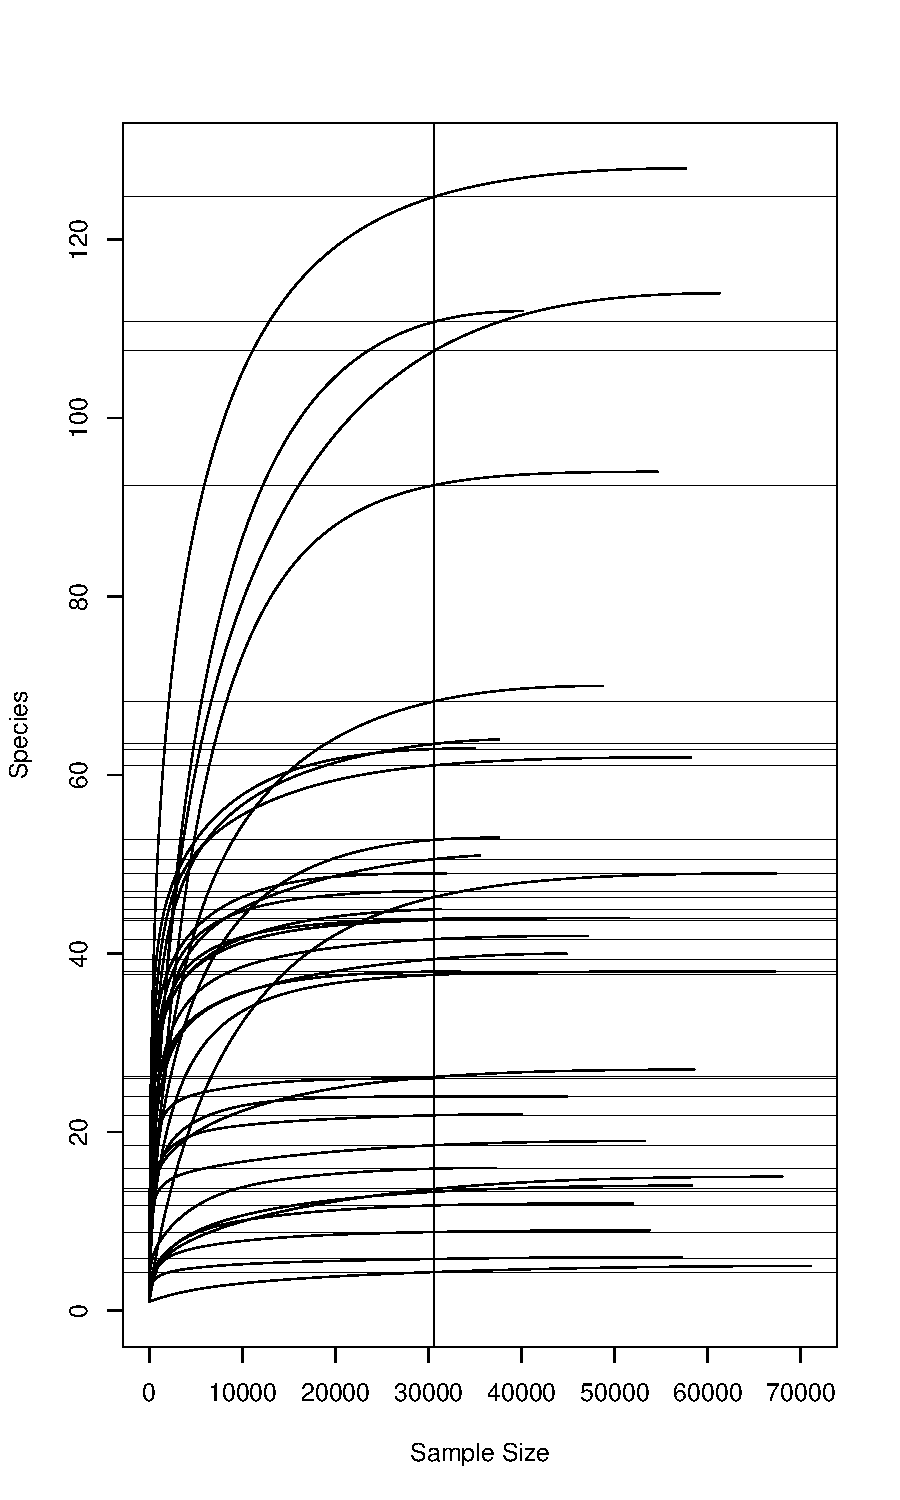
\includegraphics[width=1\linewidth]{manuscript_template_files/figure-latex/unnamed-chunk-20-3}
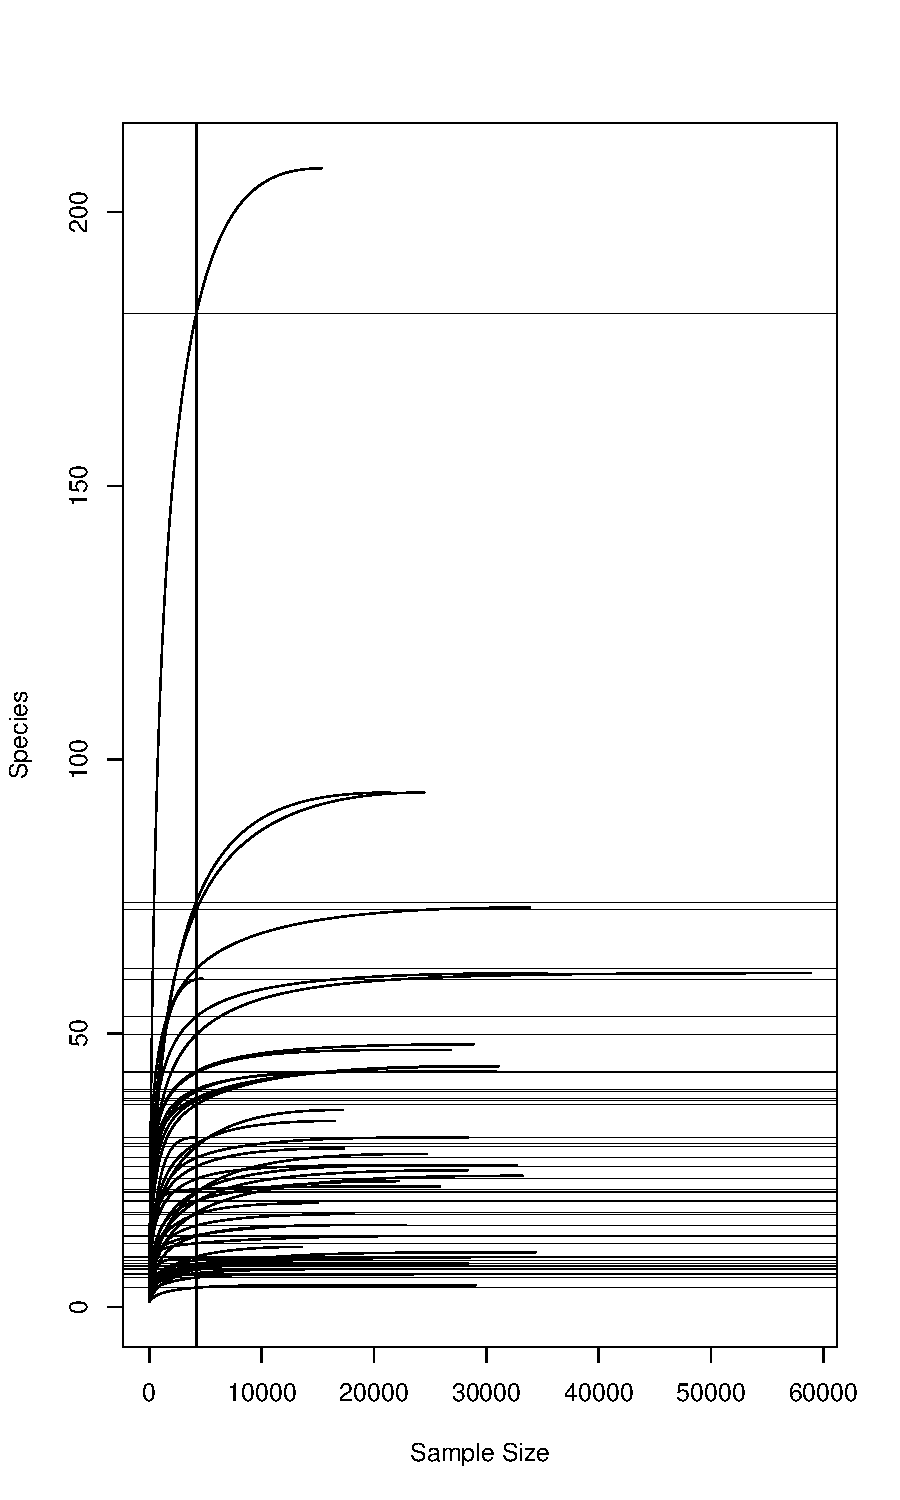
\includegraphics[width=1\linewidth]{manuscript_template_files/figure-latex/unnamed-chunk-20-4}
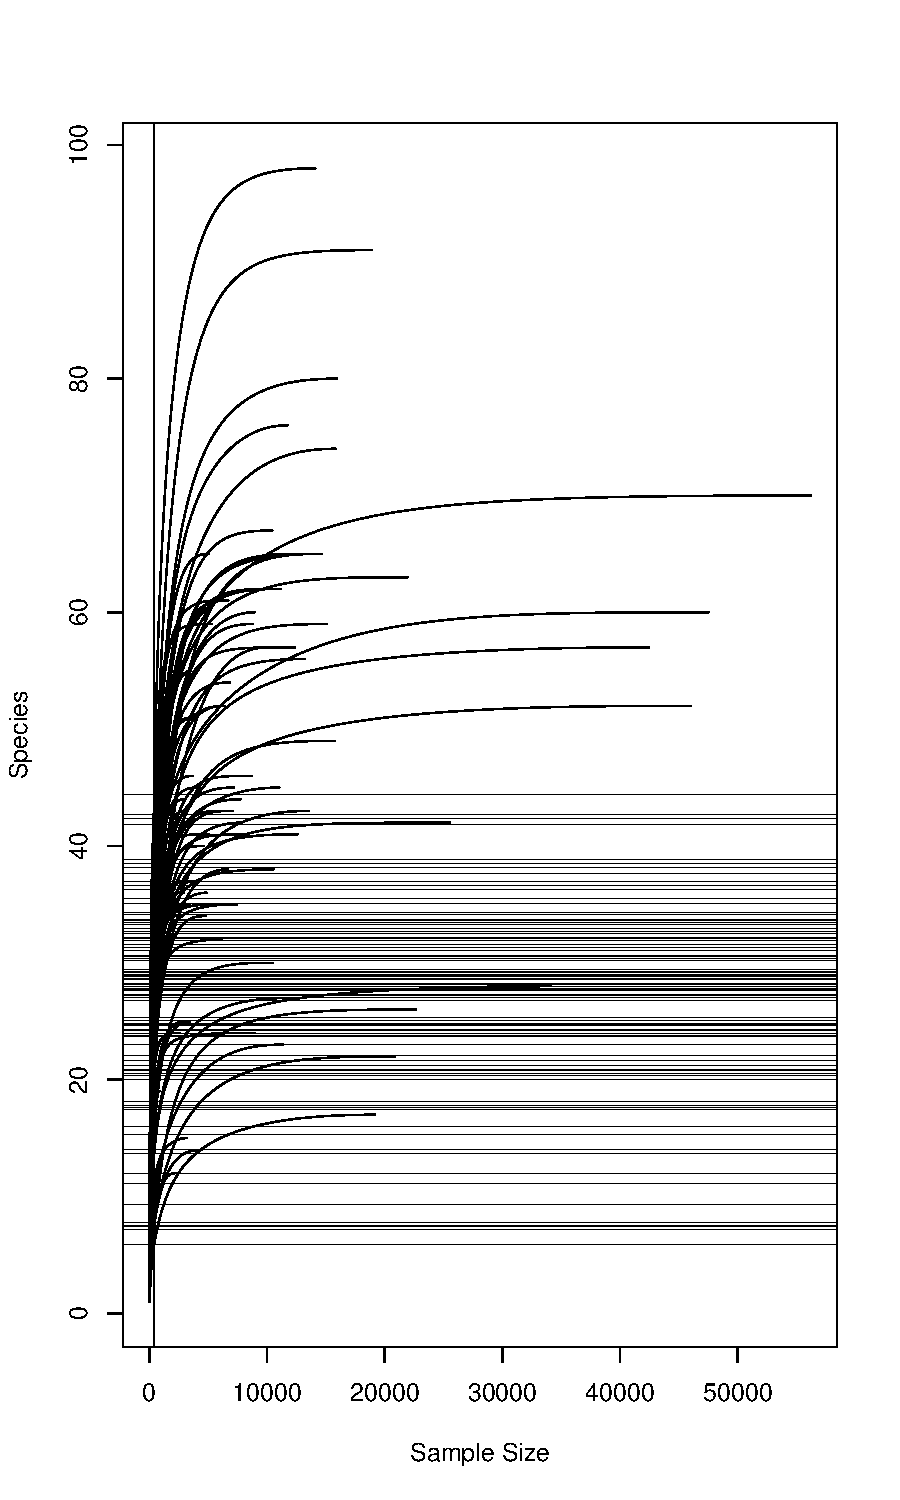
\includegraphics[width=1\linewidth]{manuscript_template_files/figure-latex/unnamed-chunk-20-5}
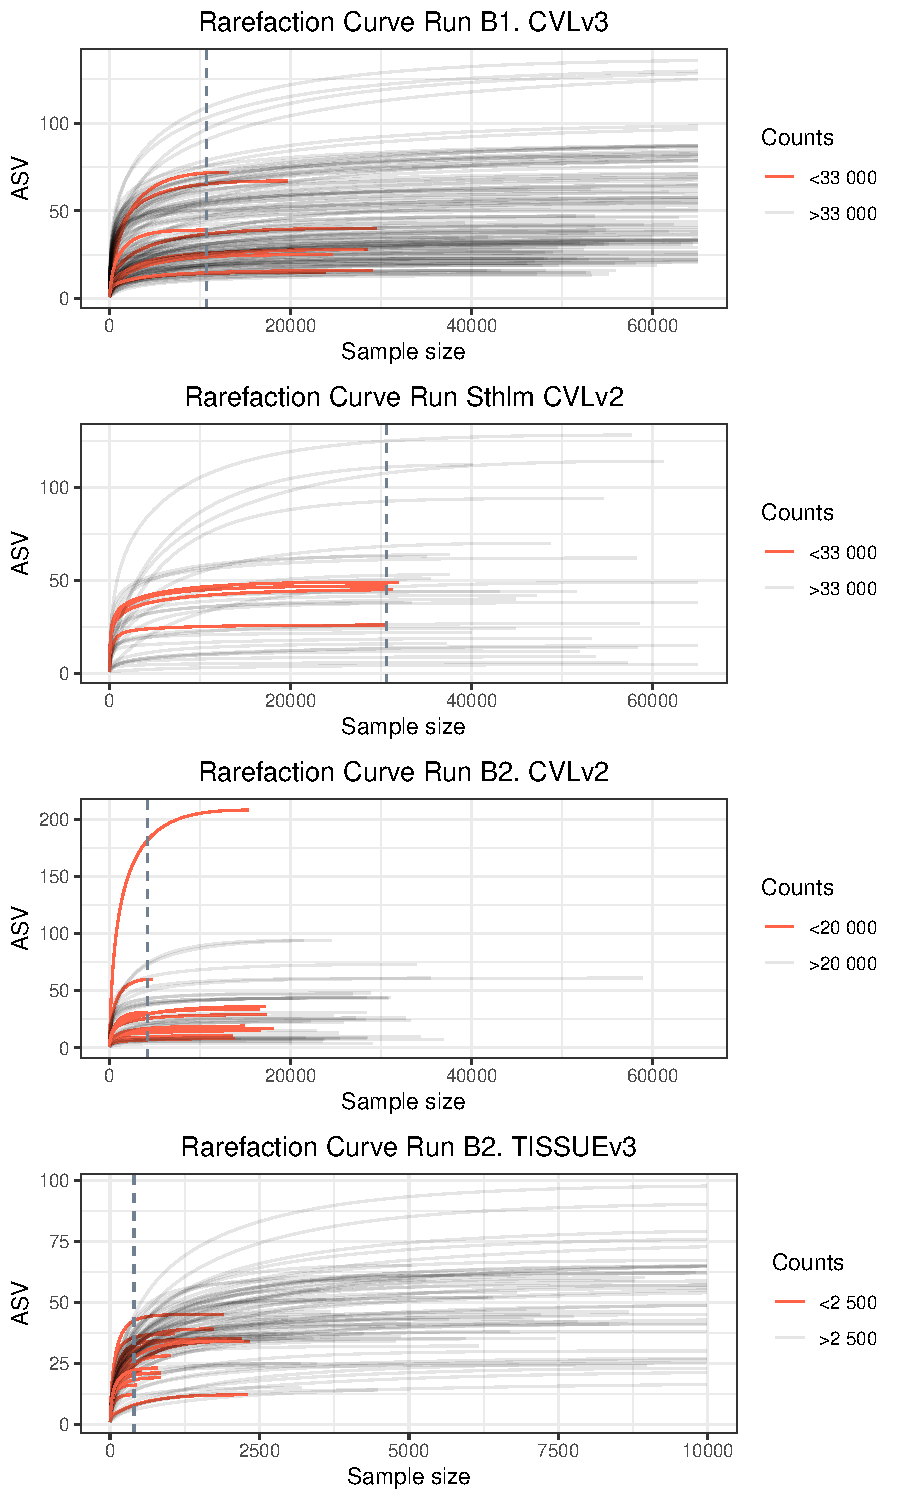
\includegraphics[width=1\linewidth]{manuscript_template_files/figure-latex/unnamed-chunk-20-6}

\clearpage

\hypertarget{tables-main}{%
\section{TABLES (MAIN)}\label{tables-main}}

\hypertarget{table-1}{%
\subsection{Table 1}\label{table-1}}

\clearpage

\hypertarget{table-2}{%
\subsection{Table 2}\label{table-2}}

\clearpage

\hypertarget{table-3}{%
\subsection{Table 3}\label{table-3}}

\clearpage

\hypertarget{tables-suppl}{%
\section{TABLES (SUPPL)}\label{tables-suppl}}

\hypertarget{table-s1}{%
\subsection{Table S1}\label{table-s1}}

\clearpage

\hypertarget{table-s2}{%
\subsection{Table S2}\label{table-s2}}

\clearpage

\hypertarget{table-s3}{%
\subsection{Table S3}\label{table-s3}}

\clearpage

\end{document}
